\documentclass[11pt]{article}
\usepackage[a4paper,margin=25mm,headheight=15pt]{geometry}
\usepackage[T1]{fontenc}
\usepackage[utf8]{inputenc}
\usepackage{lmodern,microtype}
\usepackage{amsmath,amssymb,amsthm,mathtools}
\usepackage{booktabs,longtable,tabularx,array}
\usepackage{enumitem,xcolor,graphicx,tikz}
\usepackage{fancyhdr,xurl,needspace}
\usepackage[colorlinks=true,linkcolor=navy,citecolor=teal,urlcolor=teal]{hyperref}
\definecolor{navy}{RGB}{25,49,80}
\definecolor{teal}{RGB}{0,101,106}
\definecolor{lightblue}{RGB}{235,242,247}
\hypersetup{pdftitle={Certified support and attachment-preserving product reductions for unknot recognition},
 pdfauthor={Research continuation for the ProveIt project}}
\pagestyle{fancy}
\fancyhf{}
\fancyhead[L]{\small\textsc{ProveIt / Unknot recognition}}
\fancyhead[R]{\small Certified reductions}
\fancyfoot[C]{\thepage}
\setlength{\parskip}{4pt}
\setlength{\parindent}{0pt}
\setlist{nosep,leftmargin=*}
\emergencystretch=2em
\newtheorem{theorem}{Theorem}[section]
\newtheorem{proposition}[theorem]{Proposition}
\newtheorem{lemma}[theorem]{Lemma}
\newtheorem{corollary}[theorem]{Corollary}
\theoremstyle{definition}
\newtheorem{definition}[theorem]{Definition}
\newtheorem{example}[theorem]{Example}
\newtheorem{problem}[theorem]{Research problem}
\theoremstyle{remark}
\newtheorem{remark}[theorem]{Remark}
\newcommand{\R}{\mathbb R}
\newcommand{\Q}{\mathbb Q}
\newcommand{\Z}{\mathbb Z}
\newcommand{\N}{\mathbb N}
\newcommand{\supp}{\operatorname{supp}}
\newcommand{\rank}{\operatorname{rank}}
\newcommand{\spanlin}{\operatorname{span}}
\newcommand{\cone}{\operatorname{cone}}
\newcommand{\poly}{\operatorname{poly}}
\newcommand{\nnz}{\operatorname{nnz}}
\newcommand{\bits}{\operatorname{bits}}
\newcommand{\code}[1]{\texttt{#1}}
\newcommand{\cut}{\mathbin{\backslash\!\backslash}}
\newcommand{\I}{[0,1]}
\newcommand{\Done}{\textsc{Complete}}
\newcommand{\Unknown}{\textsc{Inconclusive}}
\title{\color{navy}\bfseries Certified support and attachment-preserving\\
product reductions for unknot recognition}
\author{Research continuation for the ProveIt project}
\date{12 October 2026}
\begin{document}
\maketitle
\begin{abstract}
We develop two reductions at the present boundary between implemented
normal-surface operations and a controlled hierarchy algorithm.
The algebraic reduction determines the full feasible support of a
nonnegative matching cone before ray enumeration. Its certificate consists
of a feasible vector and a nonnegative row-space vector with complementary
supports. The certificate is checked by exact arithmetic in the original
source equations. A direct formulation in these sparse equations has an
$O(t^2)$-bit certificate for $t$ tetrahedra, without triangle elimination.
We prove an exact quotient theorem for extensions,
dual activation constraints, a sparse family invisible to bounded-size
combinations of its specified rows, and an intrinsic-dimension bound for
conflict branching.
The geometric reduction extracts the signed cyclic order of core ports
on compressed parallelity bases. Puncturing the boundary at the ports
converts ordering into endpoint matching; a second query fixes relative
fibre coordinates. Zero gaps are retained. Disc-base components consequently
admit explicit linear-size product templates preserving their labelled
attachments and the canonical first-cut seams. We provide implementations,
independent checkers, source audits, reproducible measurements, and precise
integration interfaces. The reductions remove specific sources of wasted
work and lost attaching information. The complete sector-cover and
patterned-hierarchy bounds needed for a general quasi-polynomial recognizer
remain open.
\end{abstract}
{\small\setlength{\parskip}{0pt}\tableofcontents}
\newpage

\section{The research question and the source checkpoint}
\label{sec:context}

The objective is a recognizer with a proved quasi-polynomial worst-case
bound, starting from the existing implementation in
\path{Topology/UnknotRecognition}. This requires controlling both the
search for useful surfaces and the topological representation after
cutting. A fast first cut is insufficient if the next step must expand the
surface or reconstruct its attachments from a large unstructured object.
Similarly, fast enumeration in a low-dimensional cone is insufficient if
discovering that cone requires an expensive enumeration in a much larger
space.

This article addresses these two interfaces. Its mathematical results
are stated independently of the implementations. Its experimental claims
refer only to completed measurements recorded in the package. In
particular, a supplied-sector computation, a parallelity query, and complete
unknot recognition are different tasks.

\subsection{Precisely what was inspected}

The working checkout is
\[
\text{\code{90e16db798c8d976bbe0c062e07cf20565e0b63a}}.
\]
Its relevant \code{fast/} and \code{synthesis/} trees agree exactly with the
last topology update
\[
\text{\code{e7b51c4708baefbc5836ef233301a7de3552f86b}},
\]
dated 12 October 2026. The tree identities and individual source hashes are
retained in the package manifest. This distinction matters because the
repository contains simultaneous work in other mathematical areas.

The source already contains the following ingredients
\cite{repo}:
\begin{itemize}
\item exact supplied-sector matching kernels and complete standard-ray
enumeration, including specialized geometry in dimensions at most three;
\item inexpensive sufficient forced-zero rules, and a complete feasible-span
reduction obtained \emph{after} a complete quadrilateral-ray enumeration;
\item compressed normal components, raw cuts in all cell dimensions, and
independent source reconstruction;
\item full source parallelity bases, fibre twisting, and an inherited
complementary core with at most \(30t\) handles;
\item a general exact recognition fallback, without a proved general
quasi-polynomial bound.
\end{itemize}

The first contribution avoids the expensive prerequisite in the second
item. The second makes a particular part of the fourth item's implicit
attaching information explicit and usable by a replacement operation.
The original source packet remains available as provenance.

\subsection{Literature and the meaning of the target}

Two primary versions of Lackenby's 2021 announcement state different
exponents. The February slides give
\(n^{O(\log n)}\); the March Oxford handout gives
\(2^{O((\log n)^3)}=n^{O((\log n)^2)}\)
\cite{lackenby-feb,lackenby-mar}. Both are quasi-polynomial.
The repository's attribution of the first bound to the February slides is
therefore supported. One should specify the version instead of silently
substituting the March exponent.

The July 2026 preprint supplies a hierarchy algorithm and important
compressed-decomposition results. Proposition 9.1 bounds the number of
iterations by \(L(g+1)^L\), in terms of hierarchy length and pattern
complexity; its later sections study bounded handle types and certificates
\cite{lackenby2026}. These results motivate the present interfaces.
They do not supply the missing global bound for the code studied here.

The linear-algebra foundation below is the theorem of alternatives and
rational linear programming \cite{boyd,khachiyan}. The orbit foundation is the
Agol--Hass--Thurston interval-pairing method \cite{aht}. We do not claim either
foundation, ordinary strict complementarity, or the PL classification of
a disc bundle as new. The contributions are the specific complete
certificates, transfer statements, obstruction families, compressed
port reconstruction, relative replacement specification, and their
implementation at this repository checkpoint. Priority of these derived
results in the broader literature is not asserted.

\subsection{A contribution ledger}

\begin{longtable}{@{}>{\raggedright\arraybackslash}p{.27\textwidth}>{\raggedright\arraybackslash}p{.42\textwidth}>{\raggedright\arraybackslash}p{.23\textwidth}@{}}
\toprule
Result & What it establishes & Status in this package\\
\midrule
Exact support certificate &
Every removed coordinate is impossible; every retained coordinate is
positive in one feasible vector. & Proved and implemented.\\
Direct sparse-source LP &
An original-source certificate of $O(t^2)$ bits without triangle
elimination. & Proved alternative formulation.\\
Quotient extension and dual activation &
When support can be reused, how dimension changes, and why a small column
change can still revive a large cone. & Proved; future search interface.\\
Bounded-row obstruction &
Sparse matching-like systems of arbitrarily large raw nullity evade
bounded-row sign consequences. & Proved; abstract fixtures.\\
Dimension-controlled conflict search &
A bound exponential in feasible span dimension for homogeneous
linear feasibility with quadrilateral exclusions. &
Proved; no essential-disc inference.\\
Cyclic port and fibre recovery &
The order, endpoint orientation, gap data, and relative fibre information
at core contacts. & Proved and implemented.\\
Disc product templates &
A small PL replacement relative to labelled core attachments and
canonical first-cut seams. & Proved; explicit templates emitted.\\
General quasi-polynomial recognition &
Complete useful-surface discovery and a controlled patterned hierarchy. &
Open.\\
\bottomrule
\end{longtable}

\section{Normal coordinates and the precise algebraic interface}
\label{sec:normal-interface}

Let \(t\) denote the number of tetrahedra. A standard normal vector has
four triangle and three quadrilateral coordinates in each tetrahedron.
Across each paired face, the three types of normal arcs must match.
Write these homogeneous integer equations as
\[
M_\triangle a+M_\square q=0.
\]
Nonnegativity is required. In addition, at most one quadrilateral type
can be nonzero in each tetrahedron. Throughout the supplied-sector
interface, the allowed types \(\Sigma\) already satisfy this compatibility
restriction. A coordinate may be allowed and still be forced to zero.

The existing source kernel eliminates triangle differences, retaining
vertex-link freedom, and obtains a homogeneous rational system
\[
A_\Sigma q=0,\qquad q\geq0.
\]
The relevant cone is
\[
C_\Sigma=\ker(A_\Sigma)\cap\R_{\geq0}^{k},\qquad k=|\Sigma|.
\]
Its \emph{raw nullity} is \(d=k-\rank A_\Sigma\).
Its \emph{effective dimension} is
\[
s=\dim\spanlin C_\Sigma.
\]
The two can be very different: a linear kernel contains signed directions
that may be absent from the nonnegative cone.

For this finite compact source model, a quadrilateral solution satisfying
the elimination equations admits triangle potentials. Adding sufficiently
large vertex links makes all triangle coordinates nonnegative. This
source-kernel property is already implemented and is independently
checkable through the original face equations. It is not an assertion
about arbitrary ideal or spun-normal coordinate systems.

\subsection{Why a complete support certificate changes the cost}

Let
\[
S=\{j:\text{there is }q\in C_\Sigma\text{ with }q_j>0\}.
\]
After proving that all coordinates outside \(S\) vanish, the restricted
cone has a strictly positive point. It therefore spans its whole restricted
kernel:
\[
\spanlin C_\Sigma\cong\ker A_{\Sigma,S}.
\]
Consequently the existing low-dimensional ray machinery can be dispatched
using \(s\), without first enumerating in raw dimension \(d\).

This is a substantive difference from merely assigning numerical zeros to
small coordinates in an LP solution. An LP vertex typically has many zero
coordinates that are positive elsewhere in the cone. The certificate
must prove which zeros are \emph{unavoidable}, and must prove that its
retained set is complete.

\subsection{A certificate directly in source equations}

The implementation can bind the support statement to the source without
asking the verifier to trust the producer's elimination:
\begin{enumerate}
\item supply an integral standard normal vector \(v=(a,q)\) whose
quadrilateral support is exactly \(S\);
\item supply coefficients \(\lambda\) on the original face-matching rows;
\item verify
\[
M_\triangle^{\mathsf T}\lambda=0,\qquad
y_\Sigma=(M_\square)_\Sigma^{\mathsf T}\lambda\geq0;
\]
\item verify \(q\geq0\), the original matching equations, and
\(q_j+y_j\geq1\) for every allowed quadrilateral coordinate.
\end{enumerate}
Here the nonnegativity requirement concerns only allowed columns; coefficients
on disallowed quadrilateral columns are unrestricted. For any source-feasible
standard vector \((a',q')\) in the stated sector, \(q'\) vanishes outside
\(\Sigma\), and
\[
0=\lambda^{\mathsf T}(M_\triangle a'+M_\square q')
  =y_\Sigma^{\mathsf T}q'_\Sigma.
\]
Thus every coordinate on which \(y\) is positive vanishes in every
source-feasible vector. The supplied \(q\) witnesses simultaneous positivity
on the complementary set. Triangle cancellation in the dual is essential:
without it, triangle coordinates could compensate for a positive
quadrilateral term.

Only columns in the stated sector are considered. A certificate for one
sector does not justify deleting a type in a larger sector unless the
extension conditions proved below are checked.

% Independent mathematical audit notes.  No preamble; all assertions below
% concern linear cones unless a separate geometric hypothesis is stated.
% Standard foundations: Farkas alternatives, rational LP, basic feasible
% solutions, rank-nullity, and elementary face theory.  The application and
% the explicit transfer/family statements should not be advertised as a new
% discovery of strict complementarity or polynomial-time linear programming.

\section{Complete support by one primal--dual feasibility problem}

Let $A\in\mathbb Q^{m\times k}$ and write
\[
 C(A)=\{x\in\mathbb R^k:Ax=0,\ x\geq0\},\qquad
 S(A)=\{j:\text{some }x\in C(A)\text{ has }x_j>0\}.
\]
The complement $F(A)=\{1,\ldots,k\}\setminus S(A)$ is the set of
coordinates forced to zero.  All inequalities between vectors are
coordinatewise.  A dual exposing vector means a vector
$y=A^T\lambda\geq0$ whose zero set is exactly $S(A)$.

\begin{theorem}[Complete support from a joint linear certificate]
The linear system
\begin{equation}\label{eq:audit-joint}
 Ax=0,\qquad y=A^T\lambda,\qquad x\geq0,\quad y\geq0,
 \qquad x+y\geq\mathbf1
\end{equation}
is feasible for every rational matrix $A$.  Every feasible solution has
\[
 \operatorname{supp}(x)=S(A),\qquad
 \operatorname{supp}(y)=F(A).
\]
In particular, a verifier needs only exact matrix arithmetic and sign
tests, rather than access to the optimization routine producing the
certificate.
\end{theorem}

\begin{proof}
First prove the coordinate alternative.  Let $a_j$ be column $j$ of
$A$.  There is an element of $C(A)$ with positive $j$th coordinate if
and only if
\[
 A_{-j}u=-a_j,\qquad u\geq0
\]
is feasible: scale the positive coordinate to one.  If this system is
infeasible, Farkas' lemma supplies $\lambda^{(j)}$ such that
\[
 A_{-j}^T\lambda^{(j)}\geq0,
 \qquad a_j^T\lambda^{(j)}>0.
\]
Thus $A^T\lambda^{(j)}\geq0$, with a positive $j$th coordinate.
Conversely, such a vector forces $x_j=0$ for every $x\in C(A)$, since
\[
 0=(Ax)^T\lambda^{(j)}=x^TA^T\lambda^{(j)}
\]
is a sum of nonnegative terms.  This also checks the sign in the Farkas
alternative.

For each $j\in S(A)$ choose a primal witness and scale it so its $j$th
coordinate is at least one.  Their sum $x$ is positive on every
coordinate of $S(A)$ and zero outside $S(A)$.  For each $j\in F(A)$
choose the dual witness just constructed and scale it so its $j$th
coordinate is at least one.  Sum the corresponding multipliers to obtain
$\lambda$, and set $y=A^T\lambda$.  Every summand of $y$ vanishes on
$S(A)$ by orthogonality with feasible primal witnesses.  Consequently
$x+y\geq\mathbf1$, proving existence.  Empty sums cause no difficulty.

Now consider any solution of \eqref{eq:audit-joint}.  We have
$x^Ty=0$, so nonnegativity gives $x_jy_j=0$ for each $j$.
The last inequality ensures that exactly one of $x_j,y_j$ is positive.
Every positive $x_j$ witnesses $j\in S(A)$, while every positive $y_j$
forces $j\notin S(A)$.  This proves the claimed partition.
\end{proof}

The theorem is a specialization of classical alternatives and strict
complementarity for the nonnegative orthant.  Its use here is a complete
replacement for sufficient one-row or two-row sign propagation.

\subsection{Polynomial bit complexity, including redundant rows and lineality}

\begin{proposition}[Small exact certificates]
After clearing row denominators, suppose $A$ is integral with
$|A_{ij}|\leq H$, where $H\geq1$.  System
\eqref{eq:audit-joint} has a rational solution of polynomial encoding
length in $m,k,\log H$.  More explicitly, put $v=3k+2m$ and let
$\rho\leq m+2k$ be the rank of the equality matrix in the standard-form
system below.  One may choose a common denominator and all primal and
dual variable numerators of magnitude at most
\[
 D=\rho!H^\rho,
\]
except that a multiplier $\lambda_i$ obtained as a difference of two
nonnegative variables may require the bound $2D$.  The convention
$D=1$ applies if $\rho=0$.  In particular the total number of bits is
$O(v\rho(\log(H+1)+\log(\rho+1)))$, up to ordinary bookkeeping.
\end{proposition}

\begin{proof}
Split $\lambda=\lambda^+-\lambda^-$ and introduce a nonnegative surplus
vector $z$.  All variables in
\[
 Ax=0,\qquad A^T\lambda^+-A^T\lambda^- - y=0,
 \qquad x+y-z=\mathbf1,
 \qquad x,y,z,\lambda^+,\lambda^-\geq0
\]
are nonnegative.  This is a feasible standard-form rational system
$Mu=b$, with integral coefficients bounded by $H$ and with entries of
$b$ equal to zero or one.  Remove redundant equality rows, leaving
$\rho$ independent rows.  Row removal means choosing a subset of the
original rows; it does not enlarge the coefficient bound.  Since the
system is feasible, the removed equations follow from those retained
with the correct right-hand sides.

For completeness, a nonempty standard-form feasible set has a basic
feasible solution even when the original free-multiplier formulation
has lineality.  Choose a feasible vector with minimum positive support.
If the columns of $M$ on that support were dependent, perturb within
their dependence in a direction and for a distance that makes one
positive coordinate zero while keeping all others nonnegative.  This
preserves the equalities and contradicts minimality.  The support
columns are therefore independent.  Extend them to a basis of $\rho$
columns, assigning zero to any added coordinates.  This produces a
basic feasible solution.  Equivalently, the nonnegative standard-form
feasible set contains no affine line, despite potentially unbounded
recession directions.

Cramer's rule on the corresponding $\rho\times\rho$ nonsingular
integer matrix bounds its determinant and all numerator determinants
by $\rho!H^\rho$.  The determinant is a nonzero integer.  This proves
the bounds and the claimed encoding length.  Recombining the split
multipliers introduces at most the stated factor two.

For rational $A$, clearing denominators row by row has polynomial bit
cost in its input encoding.  If $A'=RA$ is the resulting integer matrix,
where $R$ is diagonal, a multiplier $\mu$ for $A'$ corresponds to the
source multiplier $R\mu$ for $A$.  This transformation again has
polynomial encoding length.
\end{proof}

Classical rational linear-programming algorithms therefore find such a
certificate in polynomial bit time.  This statement concerns the
mathematical LP primitive; it does not assert a polynomial pivot bound
for a chosen simplex implementation.  Clearing a common positive
denominator in a joint certificate also produces integral $x,y,\lambda$:
the inequality $x+y\geq\mathbf1$ becomes stronger after this scaling.

\section{The support restriction is the intrinsic linear span}

\begin{proposition}[Effective dimension]
Let $S=S(A)$.  Extension by zero gives a cone isomorphism
\[
 C(A_S)\longrightarrow C(A),
\]
and
\[
 \operatorname{span} C(A_S)=\ker A_S,
 \qquad \dim\operatorname{span} C(A)=|S|-\operatorname{rank} A_S.
\]
\end{proposition}

\begin{proof}
All deleted coordinates vanish on $C(A)$, so restriction and extension
by zero are inverse linear maps on the cones.  There is a vector
$p\in\ker A_S$ with $p>0$.  Given $u\in\ker A_S$, choose
$\epsilon>0$ small enough that $p\pm\epsilon u\geq0$.  Both of these
vectors belong to $C(A_S)$, and their difference is $2\epsilon u$.
This proves the span assertion.  Rank-nullity gives the formula.
\end{proof}

Extension by zero also preserves the complete face lattice, extreme
rays, linear objectives and the integral lattice in these coordinate
spaces.  More generally it preserves any further conditions on the
retained coordinates.  When applying this to normal surfaces, one must
still justify the relationship between the matching cone used for
support computation and the actual standard-coordinate source cone.
Forced zeros in a relaxation safely remain forced in every geometric
subcone; maximality in a relaxation does not establish maximality after
quadrilateral exclusions or other geometric restrictions.

\section{Exact reuse when allowed columns are deleted or added}

Throughout this section, all columns belong to one fixed matrix of
source constraints.  The results do not authorize reuse across a
Pachner move or any other change to the source equations without a
separate transport proof.  Write $C_I=C(A_I)$ for an allowed column set
$I$.  Let $S=S(A_I)$, $F=I\setminus S$, and choose a complete exposing
multiplier $\lambda$ such that
\[
 y_i=a_i^T\lambda=0\ (i\in S),\qquad
 y_i>0\ (i\in F).
\]

\subsection{Deletion and lifting a smaller dual certificate}

\begin{proposition}[Restriction and dual lifting]
For $I'\subseteq I$, every coordinate of $F\cap I'$ remains forced
zero.  Complete support for $I'$ may therefore be computed using only
$R=S\cap I'$.  If $I'$ contains $S$, the original support and effective
dimension are unchanged.  In general the effective dimension cannot
increase.

Suppose $\eta$ is a complete exposing multiplier for the smaller cone
$C(A_R)$, and put $v_i=a_i^T\eta$ for all $i\in I'$.  Define
\[
 \alpha=1+\max_{i\in F\cap I'}
              \frac{\max(0,-v_i)}{y_i},
\]
where the maximum of an empty set is zero.  Then
$\eta+\alpha\lambda$ is a complete exposing multiplier on $I'$.
All these operations preserve polynomial certificate bit length.
\end{proposition}

\begin{proof}
The restriction of $y$ is still a nonnegative row-space consequence,
so its positive coordinates remain zero on every feasible vector.
This gives the cone isomorphism with $C(A_R)$.  The cone for $I'$ is a
coordinate face of the old cone, embedded with zeros, so its dimension
cannot increase.  If only old forced coordinates are deleted, the cones
are identical under that embedding.

On $R$, the old exposing vector is zero, so the new exposing vector
equals $v$.  On $F\cap I'$, its coefficient is
$v_i+\alpha y_i\geq y_i>0$.  Its zero set is therefore precisely the
new maximal support.  Rational maxima, products and quotients of the
displayed certificate entries have polynomial bit length.
\end{proof}

\subsection{Which added columns can invalidate an exposing vector?}

\begin{theorem}[Dual sign test for extensions]
Add columns indexed by $E$, disjoint from $I$, and let
\[
 w_e=a_e^T\lambda,\qquad
 E_+=\{e:w_e>0\},\quad E_0=\{e:w_e=0\},\quad
 E_-=\{e:w_e<0\}.
\]
Every $q\in C_{I\cup E}$ satisfies the exact balance identity
\begin{equation}\label{eq:audit-portal}
 \sum_{i\in F}y_iq_i+\sum_{e\in E_+}w_eq_e
       =\sum_{e\in E_-}(-w_e)q_e.
\end{equation}
Consequently, positive use of an old forced coordinate or of a column
in $E_+$ requires positive use of at least one column in $E_-$.

If $E_-=\varnothing$, every coordinate in $F\cup E_+$ is still forced
zero, and the expanded cone is isomorphic to $C(A_{S\cup E_0})$.
Writing $d=\dim\operatorname{span}C_I$ and $d'$ for the corresponding
dimension after extension, one has
\[
 d\leq d'\leq d+|E_0|.
\]
If every added column has strictly positive $w_e$, the old cone and
support remain unchanged.
\end{theorem}

\begin{proof}
Apply $\lambda^T$ to the matching equation for $q$ and move its negative
terms to the other side.  This proves \eqref{eq:audit-portal}.
Every summand on both sides is nonnegative, giving the necessity
statement and, when $E_-$ is empty, all asserted forced zeros.
Old feasible vectors extend by zero, so $d'\geq d$.  Since
$\dim\ker A_S=d$, adding $|E_0|$ columns increases the kernel dimension
by at most $|E_0|$.  The new feasible span lies in that kernel, yielding
the upper bound.  The last assertion follows when $E_0$ is empty.
\end{proof}

\begin{example}[One added column can cause arbitrary revival]
Let $A_I=(1,\ldots,1)$ have $r$ columns.  Its nonnegative kernel is
zero.  Add the single column $-1$.  The new cone is
\[
 \{(u_1,\ldots,u_r,t)\geq0:t=u_1+\cdots+u_r\},
\]
which has all $r+1$ coordinates in its maximal support and dimension
$r$.  The old multiplier $\lambda=1$ evaluates negatively on the added
column.  Thus no dimension bound depending only on the old effective
dimension and the number of added columns can hold without additional
hypotheses.  In particular the nonnegative sign hypothesis above is
substantive.
\end{example}

\subsection{Contracting the live core}

\begin{theorem}[Quotient extension and exact dimension sequence]
Let $S$ be a column set admitting $p>0$ with $A_Sp=0$.  Set
$V=\operatorname{im}A_S$, and choose an exact linear map $Q$ with
$\ker Q=V$.  For any allowed set $J\supseteq S$, put
\[
 R=J\setminus S,\qquad B=QA_R.
\]
The coordinate projection onto $R$ maps $C(A_J)$ surjectively onto
$C(B)$.  If $U=S(B)$, then
\[
 S(A_J)=S\cup U.
\]
There is a short exact sequence of real vector spaces
\[
 0\longrightarrow\ker A_S
   \xrightarrow{\;u\mapsto(u,0)\;}
   \operatorname{span}C(A_J)
   \xrightarrow{\;\pi_R\;}
   \operatorname{span}C(B)
   \longrightarrow0.
\]
Hence the effective dimensions satisfy the exact additive identity
\[
 \dim\operatorname{span}C(A_J)
       =\dim\ker A_S+\dim\operatorname{span}C(B).
\]
All matrix constructions can be performed in polynomial rational bit
time.  The theorem includes $S=\varnothing$, with $V=0$ and a vacuous
positive vector.
\end{theorem}

\begin{proof}
First observe that the columns in $S$ positively generate their entire
linear span: if $A_Su=v$ for signed coefficients $u$, then
$A_S(u+cp)=v$, and $u+cp\geq0$ for all sufficiently large $c$.
Thus $\operatorname{cone}(A_S)=V$.

If $(x,z)\in C(A_J)$, applying $Q$ gives $Bz=0$, so the projection is
well-defined.  Conversely, let $z\geq0$ satisfy $Bz=0$.  Then
$A_Rz\in V$, so choose signed $u$ with $A_Su=-A_Rz$.  For sufficiently
large $c$, $u+cp\geq0$ and $(u+cp,z)\in C(A_J)$.  This proves
surjectivity on the cones.  Every coordinate of $S$ remains feasible
by embedding the original positive vector; surjectivity determines
exactly which coordinates of $R$ are feasible.  This proves the
support identity.

The injection in the displayed sequence is well-defined because
$\ker A_S=\operatorname{span}C(A_S)$ and $C(A_S)$ embeds into
$C(A_J)$.  Surjectivity of the last arrow follows by taking spans of
the already established cone surjectivity.  A vector in the middle
space with zero $R$ coordinates has form $(u,0)$, and its matching
equation says $A_Su=0$.  Conversely every such vector belongs to the
image of the first arrow.  This proves exactness and therefore the
dimension formula.

An exact basis of the annihilator of $\operatorname{im}A_S$ provides
$Q$.  Standard rational elimination and its minor bounds give the
stated construction and bit bounds.
\end{proof}

This quotient construction preserves the linear nonnegative cone.
If $J$ contains mutually incompatible quadrilateral types, the lift by
$cp$ may use incompatible types; the theorem then describes a safe
matching relaxation and does not itself solve the compatibility
problem.  For a compatible fixed sector, this particular obstruction
does not occur, although the separate geometric verification remains.

\section{Sparse families separating raw and effective dimension}

\begin{theorem}[Cyclic obstruction to bounded-row sign propagation]
Fix integers $m\geq3$ and $s\geq1$.  Use nonnegative variables
$p_1,\ldots,p_m,z_1,\ldots,z_m,t_1,\ldots,t_{s-1}$, with cyclic
indices on the $z$ variables, and impose
\[
 p_i+z_i-z_{i+1}=0\qquad(1\leq i\leq m).
\]
In the displayed variable ordering the matrix is already in reduced
row-echelon form.  Its rank is $m$ and its raw matching nullity is
$m+s-1$.  Its nonnegative cone has maximal support consisting of all
$z$ and $t$ coordinates and has effective dimension $s$.

Every nonzero nonnegative linear combination of the displayed rows
uses all $m$ rows.  Here ``nonnegative linear combination'' means a
row combination whose resulting coefficients are all nonnegative;
the combination's multipliers are not assumed nonnegative in advance.
Thus any sign-forcing method examining only spans of at most $h<m$
of these rows makes no first step and therefore no progress.
\end{theorem}

\begin{proof}
The $p$ columns form the identity matrix, proving the rank and RREF
claims.  Sum all equations to obtain $\sum_i p_i=0$.  Nonnegativity
forces $p_i=0$ for every $i$, after which the equations require all
$z_i$ to be equal.  The common value and the $s-1$ free $t$ values
parameterize the cone as $\mathbb R_+^s$.  Setting the common value
and all free values to one proves the support statement.

For a row combination with multipliers $\lambda_i$, the $p_i$
coefficient is $\lambda_i$, so a nonnegative resulting row requires
$\lambda_i\geq0$.  Its $z_i$ coefficient is
$\lambda_i-\lambda_{i-1}$.  All these coefficients are nonnegative
and their sum is zero.  They are therefore all zero, forcing all
$\lambda_i$ to be equal.  A nonzero nonnegative result consequently
has every multiplier strictly positive and uses all $m$ rows.
No bounded-row sign step is initially available, so there are no
earlier forced zeros from which an iterative closure could begin.
\end{proof}

An exact joint certificate is particularly small:
\[
 x_p=0,\quad x_z=\mathbf1,\quad x_t=\mathbf1,
 \qquad \lambda=\mathbf1,
 \qquad y_p=\mathbf1,\quad y_z=y_t=0.
\]
Every row has three nonzero entries, and every matrix entry is in
$\{-1,0,1\}$.  For fixed $s$, the raw dimension tends to infinity
while the complete support reduction exposes a fixed-dimensional
feasible cone.

The obstruction is deliberately relative to the specified row family,
including its RREF presentation.  It is not invariant under arbitrary
change of row basis: a basis containing the sum of all rows would
immediately reveal the forced zeros.  That dependence is exactly why
fixed one-row and two-row closure is insufficient.

\begin{example}[A bounded-coefficient variant with effective dimension zero]
Replace the cyclic equations by
\[
 p_i-z_i+2z_{i+1}=0.
\]
Their sum forces all $p_i,z_i$ to vanish, so the nonnegative cone is
zero despite raw nullity $m$.  A nonnegative row consequence has
$\lambda_i\geq0$ and $\lambda_i\leq2\lambda_{i-1}$.  If one
multiplier vanishes, these cyclic inequalities force every multiplier
to vanish.  Thus every nonzero nonnegative consequence again uses all
$m$ rows.  Appending $s$ unconstrained nonnegative columns gives raw
nullity $m+s$ and effective dimension $s$, for any $s\geq0$.
\end{example}

These are structural examples for abstract rational matching systems.
No realization by triangulated knot exteriors, or by the repository's
actual source-derived sector equations, is asserted.  They establish
an algebraic separation and supply regression cases; a geometric
realization theorem would be additional research.

\section{Conflict branching controlled by intrinsic dimension}

\begin{theorem}[A dimension bound for compatibility search]
Let $A$ and $\ell$ be rational, and let $\mathcal P$ be a set of
forbidden coordinate pairs.  Consider the decision problem
\[
 Ax=0,\quad x\geq0,\quad \ell^Tx>0,
 \qquad x_ix_j=0\quad\text{for every }\{i,j\}\in\mathcal P.
\]
Put $d=\dim\operatorname{span}C(A)$, and let $N$ be the bit length of
the rational input and pair list.  Following complete support
restriction, this problem can be solved using at most
$2^{d+1}-1$ additional linear-feasibility queries, each of polynomial
bit complexity in $N$.  Its total bit running time is
$2^{O(d)}\operatorname{poly}(N)$.
In particular $d=O(\log N)$ gives a polynomial bound, and
$d=O((\log N)^2)$ gives $N^{O(\log N)}$.
\end{theorem}

\begin{proof}
Use homogeneity to replace $\ell^Tx>0$ by $\ell^Tx\geq1$.
At a search node retain the matching equations, nonnegativity and
the coordinate-zero equations selected along its path.  Query
feasibility with $\ell^Tx\geq1$.  An infeasible node is rejected.
If a feasible witness has no forbidden pair positive, it solves the
problem.  Otherwise choose a forbidden pair $\{i,j\}$ whose two
coordinates are positive in this witness and branch on $x_i=0$ and
$x_j=0$.  Every compatible feasible vector belongs to at least one
child, so the branching is complete.

Let $C_v$ be the homogeneous matching cone at a feasible node.
The coordinate functionals $x_i$ and $x_j$ are both nonzero on
$\operatorname{span}C_v$, as witnessed by the positive conflicting
coordinates.  Each child cone is contained in the kernel of one of
these nonzero functionals.  Consequently each child has span
dimension at most $\dim\operatorname{span}C_v-1$; the child is also
a proper coordinate face of $C_v$.  At depth $d$ every remaining
cone is zero, so its normalized LP is infeasible.  A binary tree of
depth at most $d$ has at most $2^{d+1}-1$ nodes.

All node systems consist of the original input and coordinate-zero
conditions, so their input bit lengths remain polynomial in $N$.
Rational linear programming supplies the required polynomial cost per
query.  The displayed complexity consequences follow directly.
\end{proof}

It is enough to compute complete support once at the root: its
restricted kernel has dimension exactly $d$.  Recomputing support at
children can improve practical pruning and dimension estimates but is
unnecessary for the bound.  Similarly, a zero-dimensional homogeneous
cone can be rejected before an LP call, improving constants but not
the theorem's stated bound.

Quadrilateral exclusions are represented by the three forbidden pairs
among the three quadrilateral types of each tetrahedron.  The theorem
is a refinement of familiar LP-guided compatibility branching, not an
assertion that such branching was previously unknown.  Its useful
parameter is the intrinsic matching-cone dimension exposed by the
complete support certificate.

This theorem is an algebraic existence result.  An arbitrary positive
linear objective does not imply an essential normal disc.  Even when
the objective is Euler characteristic in genuine standard normal
coordinates, vertex links, spheres, disconnected components and
boundary-parallel discs require the applicable established geometric
arguments and verification steps.  Nor has a logarithmic-squared
bound on $d$ for arbitrary knot-exterior inputs been proved here.


\section{Implementing source support certificates}
\label{sec:support-implementation}

\subsection{Producer and independent checker}

The new producer accepts either an explicit rational matrix or a source
triangulation with compatible allowed quadrilateral types. In the generic
interface the mathematical certificate is a pair \((x,\lambda)\).
In the source interface it is a normal vector together with coefficients
on the source face equations. The independent checker verifies exact
matrix products, signs, support coverage, and source identity. It does not
accept a numerical LP status as a proof.

The current source validator accepts finite, connected, compact, orientable
3-manifold triangulations with exactly one torus boundary component.
It checks this source class directly; it does not establish provenance
from a knot diagram. The abstract rational-cone theorems have no such
topological restriction. The same source-class restriction applies to
the geometric APIs used below.

The automatic search path uses floating-point linear programming to
propose a support partition and candidate witnesses. Exact reconstruction
then solves the corresponding rational equations; the result is accepted
only if the full certificate passes. An exact rational simplex path is
also available. The implementation details and tested solver modes are
recorded with the experiments.

This distinction separates three claims that are easy to confuse:
\begin{itemize}
\item a complete mathematical certificate always exists;
\item rational linear programming admits polynomial-time algorithms;
\item the particular numerical or simplex producer in this package has
no claimed polynomial worst-case running time.
\end{itemize}
The verifier is independent of that last issue. Failure to find or
reconstruct a certificate produces \Unknown, not an exclusion.

\Needspace{11\baselineskip}
\subsection{A direct sparse-source formulation}

\begin{corollary}[A direct source LP with small coefficients]\label{cor:direct-source-support}
For a finite triangulation with $t$ tetrahedra and a compatible set of
$k\leq t$ allowed quadrilateral types, maximal quadrilateral support has
an original-source primal--dual certificate of $O(t^2)$ bits,
obtainable by rational linear programming without triangle elimination.
\end{corollary}
\begin{proof}
Retain all $4t$ triangle columns and the $k$ allowed quadrilateral columns
in the original matching matrix $M_\Sigma$.  It has $p\leq5t$ columns,
$m\leq6t$ rows and entries of absolute value at most $2$: each paired
face contributes three equations, each comparing a triangle-plus-quad
arc count on its two sides.  Every row has at most four nonzero entries;
every column has at most four, since a triangle has three face arcs and
a quadrilateral four.  Self-gluings can identify or cancel these
incidences and do not increase their number.
The vector $u=(\mathbf1_{4t},0_k)$ satisfies
$M_\Sigma u=0$.  Hence every triangle coordinate belongs to maximal
support, and every $y=M_\Sigma^{\mathsf T}\lambda\geq0$ satisfies
$0=u^{\mathsf T}y$, forcing all its triangle coefficients to vanish.
The joint support LP therefore directly gives the required source dual
and a nonnegative standard primal vector in the stated sector.
Its standard form has at most $3p+2m\leq27t$ nonnegative variables and
equality rank $\rho\leq m+2p\leq16t$.  Its three row types have at most
$4$, $9$ and $3$ nonzero entries, all of absolute value at most $2$;
their Euclidean norms are therefore at most $6$.  Choose independent
original equality rows and a basic feasible solution as above.  The
square basis matrix has determinant of absolute value at most $6^\rho$
by Hadamard's inequality.  In a Cramer numerator, replacing a column by
the right-hand side in $\{0,1\}^{\rho}$ raises each squared row norm by
at most one, so every such numerator has absolute value at most $7^\rho$.
All reduced denominators divide the same basis determinant; clearing
the primal denominators therefore preserves the numerator bound.
Taking the difference of split dual multipliers introduces at most a
factor of two.  Thus every certificate entry has $O(t)$ bits, and its
$O(t)$ entries require $O(t^2)$ bits in total, including row and column
indices.  Zero extension restores
the primal's disallowed quadrilateral coordinates; the multipliers
already refer to the original source rows.
\end{proof}

This is a certificate-existence result and an alternative theoretical
LP formulation.  The producer benchmarked in this package uses the
quadrilateral quotient.  The full standard kernel retains vertex-link
directions, so its dimension must not replace the effective quadrilateral
dimension used for low-dimensional dispatch; that dispatch still uses
the quotient.  The witness bound is an existence bound, not a bound on
arbitrary solver outputs or a performance claim for an implemented
direct-source solver.


\subsection{The opt-in sector wrapper}

After successful verification, the wrapper rebuilds the existing source
kernel on the retained allowed types. This preserves the exact matching
geometry and canonical lifting behavior. It then calls the ordinary
supplied-sector discovery machinery.

For a positive result, the disc certificate still concerns the actual
source triangulation and full normal coordinates. For a negative
supplied-sector result, the support certificate and the reduced-sector
exhaustion must both be retained. The first proves that every feasible
vector in the requested sector lies in the reduced sector. The second
proves that the reduced sector has been completely searched. Together
they establish coverage of the originally requested sector. A capped
ray search does not satisfy the second premise.

This package adds an explicit opt-in interface. It does not alter the
existing default recognition policy. The measured overhead on easy
sectors is one reason to preserve that choice.

\subsection{Cancellation and numerical failure}

The producer's own reconstruction, source traversal, and verification
loops accept cancellation checks. Calls into a third-party LP solver
are checked at their boundaries; the package does not claim that a
long solver call cooperatively interrupts at every internal pivot.
The reproducibility notes state this limitation explicitly.

No floating-point tolerance licenses a removal. A support proposed by a
numerical solution can be wrong because of scaling, degeneracy, or a tiny
coordinate; the exact primal--dual conditions reject it. This makes
aggressive numerical proposal generation compatible with exact
downstream certificates.

\section{Compressed parallelity and the missing order information}
\label{sec:geometry-interface}

After cutting along a normal surface \(F\), the current source constructor
describes selected product handles of indices zero, one, and two.
They form an interval bundle \(E\to B\), together with a complementary
core \(K\). A core port is a labelled free base edge whose interval product
meets a particular core chart. Original-boundary free edges are retained
separately.

The base is encoded by polygon families and interval pairings. If a
normal coordinate has \(B\) bits, a family can represent exponentially
many polygons while storing only its binary endpoints. The existing
summary records Euler characteristic, boundary count, orientability,
and the set of core ports on each connected base component. It does not
explicitly list the cyclic order of those ports along each boundary
circle.

That order is already implicit in the complete source geometry. The
problem is to extract it without expanding the polygons.

\subsection{The topological information that must survive}

The output needed for a replacement is more precise than a port set.
It includes:
\begin{enumerate}
\item the cyclic sequence of port labels;
\item the entry and exit endpoint of every traversed port;
\item whether each complementary gap is a point or a nonempty arc;
\item the relative identification of the two fibre endpoints at the ports;
\item the original source chart for every contact with the core.
\end{enumerate}

A zero gap means that neighboring port closures meet. Replacing it by a
positive gap changes the attachment subset. A fibre reversal may not be
visible in a singleton integer rank map. It must be carried as a separate
bit. These two details are indispensable even when all bases are discs.

\begin{example}[An unordered profile does not determine a marked disc]
Take an oriented disc with four labelled boundary ports, each separated
from its neighbors by a nonempty unmarked gap. The cyclic words
\[
(1,2,3,4)\quad\text{and}\quad(1,3,2,4)
\]
have the same Euler characteristic, the same boundary count, and the
same port set. No homeomorphism between the discs that preserves each
port label carries one marking to the other: boundary homeomorphisms
preserve cyclic order up to reversal. The example concerns the labelled
relative attachment problem; it need not distinguish the unlabelled
homeomorphism type of the resulting ambient 3-manifold.
\end{example}

\begin{figure}[ht]
\centering
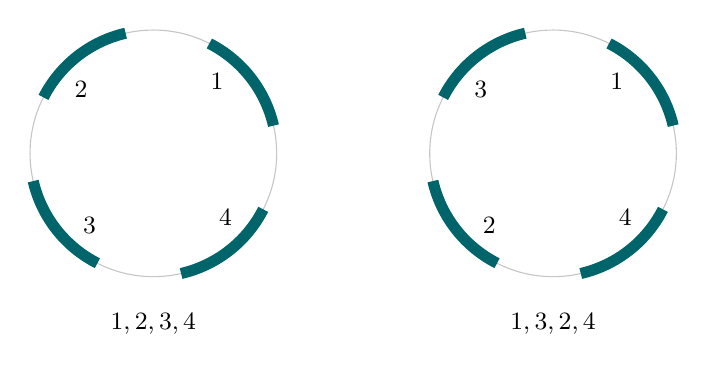
\begin{tikzpicture}[scale=1.08]
\foreach \cx/\lab in {0/{1,2,3,4},4.7/{1,3,2,4}} {
  \draw[gray!45] (\cx,0) circle (1.45);
  \foreach \ang in {0,90,180,270} {
    \draw[line width=4pt,teal] (\cx,0) ++(\ang+13:1.45)
       arc[start angle=\ang+13,end angle=\ang+63,radius=1.45];
  }
}
\node at (.75,.85) {\small 1};
\node at (-.85,.75) {\small 2};
\node at (-.75,-.85) {\small 3};
\node at (.85,-.75) {\small 4};
\node at (5.45,.85) {\small 1};
\node at (3.85,.75) {\small 3};
\node at (3.95,-.85) {\small 2};
\node at (5.55,-.75) {\small 4};
\node at (0,-2) {\small \(1,2,3,4\)};
\node at (4.7,-2) {\small \(1,3,2,4\)};
\end{tikzpicture}
\caption{The same four ports can have inequivalent cyclic attachment
data. Green arcs are labelled ports; gray arcs are nonempty gaps.
The diagrams specify cyclic order only.}
\label{fig:ports}
\end{figure}

% Integration notes: theorem statements and proofs, without a document preamble.
% Suggested bibliography: Agol--Hass--Thurston 2006; retained Lackenby July 2026
% manuscript, plus source repository synthesis/parallelity.tex.

\section{Recovering the attaching order of compressed parallelity bundles}
\label{sec:port-order}

The existing source parallelity operator retains complete polygon charts, an
inherited core with at most $30T$ handles, and at most $q\leq66T$ labelled
core ports.  Its component profiles contain Euler characteristic, boundary
count, fibre twisting and a set of port labels.  These are not yet an explicit
small attaching diagram.  In particular, a set of ports does not specify their
cyclic order.  We give an exact extraction of this order and then a relative
replacement theorem for disc products.  This operation fills a specific
geometric gap between a compressed cut and a small patterned handle structure;
it does not assert that the resulting handle structure is admissible.

\subsection{The marked boundary model}

Let $B$ be a finite, possibly disconnected, compact surface supplied as
polygons with pairwise glued sides.  We assume that the quotient really is a
surface, including the interval-or-circle condition on every vertex link.
Each unglued side lies on $\partial B$.  Select $q$ unglued side occurrences,
with distinct labels $0,\ldots,q-1$, called \emph{ports}.  Every port carries
an ordered endpoint chart $(j,0),(j,1)$.  Endpoints of different ports may
coincide after quotienting; even the two endpoints of one boundary edge cell
may coincide.  The statement concerns labelled edge parametrisations, and
does not assume that the closure of each edge cell has distinct endpoints.
All other boundary edges are called ordinary.  In the source application,
ordinary edges lie on the original manifold boundary.

The polygon families and their gluings are represented by affine interval
pairings.  Let $N$ be the number of corner occurrences before quotienting,
and let $R_V$ be the interval equivalence relation that identifies corners
across glued polygon sides.  Thus the $R_V$-orbits are the vertices of $B$.
Let $R_\circ$ be generated by $R_V$ and the endpoint pairings of every
ordinary boundary edge, \emph{omitting the port edges}.  In a compressed
family the omission of a singleton port can be achieved by splitting that
family at its rank, so $q$ omissions create only $O(q)$ additional records.
The source packet already lists each port as a singleton.

\begin{theorem}[Punctured boundary matching]
\label{thm:punctured-boundary-matching}
Give corner occurrence $(j,e)$ the weight $2^{2j+e}$ in the first coordinate.
Give exactly one endpoint occurrence of each ordinary boundary edge weight
$1$ in a second coordinate.  Weights at coincident occurrences add.  Then the
weighted orbit histogram for $R_\circ$ determines all boundary circles
containing ports, their cyclic port order, the entry endpoint of each port,
and the number of ordinary edges in each gap between consecutive ports.
No polygon or boundary-edge family needs to be expanded.

More precisely, every orbit with nonzero first coordinate has weight
\[
  \bigl(2^a+2^b,\,\ell\bigr),\qquad a\ne b,\quad\ell\geq0,
\]
and multiplicity one.  These orbits give a perfect matching $\tau$ on the
$2q$ endpoint tokens.  Let $\iota(2j+e)=2j+1-e$ pair the ends of each port.
Alternating $\iota$ and $\tau$ gives exactly the boundary circles containing
ports.  The matching edge of $\tau$ carries the intervening length $\ell$.
\end{theorem}

\begin{proof}
First quotient by $R_V$.  The free edges form the ordinary boundary
1-manifold of $B$, a disjoint union of circles.  Remove the interiors of its
$q$ port edges.  Each boundary circle containing a port becomes a union of
closed paths, possibly reduced to a single vertex.  Every such path has
exactly two incident endpoint \emph{occurrences} from the removed edges.
This remains true when consecutive ports share a vertex or a one-edge
boundary circle loses its only edge.  A circle without ports remains a
circle and carries no endpoint mark.  Interior vertices of $B$ also carry
no endpoint mark.

The connected components just described are precisely the marked
$R_\circ$-orbits.  Each endpoint bit was placed once, so a marked orbit has
exactly the two stated bits and multiplicity one.  Its second coordinate
counts ordinary boundary edges because every such edge contributes exactly
one unit to its component.  Hence this coordinate is zero exactly for a
zero-length gap; it is positive for an actual interval of ordinary boundary.
Restoring each deleted port joins its two endpoints by $\iota$, and restores
the original circles.  Walking these circles reads their port order and the
direction of each endpoint chart.  This is precisely the alternating walk
in the union of the two perfect matchings.
\end{proof}

There are two directed alternating cycles on endpoint tokens for each
unoriented boundary circle.  The implementation visits each port once, rather
than counting both cycles.  Its canonical choice starts at the least port
label on a circle, enters that port at endpoint $0$, and follows the resulting
direction.  The endpoint labels fix this direction even when the underlying
surface has no selected orientation.  With $q=0$ the output is the empty
list.  Unmarked boundary circles continue to be counted by the source
surface-classification packet, and are not spuriously returned as marked
circles.

For verification it is insufficient to compare only the sum of all endpoint
integers: duplicated bits can carry in binary arithmetic.  The checker
requires two set bits in each nonzero mask, multiplicity one, pairwise
disjoint endpoint-token sets, and their union equal to all $2q$ tokens.
The underlying source-bound construction also authenticates that each mark
was placed at exactly its specified source corner occurrence.

\subsection{Relative fibre charts}

Let $E\to B$ be the source $I$-bundle.  Each polygon has a local product
chart, and every side gluing specifies whether it reverses the fibre.
These signs define the fibre-orientation double cover $\widetilde B\to B$.
The existing source packet checks that they arise from the actual source
bundle.  In particular, they are compatible around vertices; arbitrary
signs on a polygon adjacency graph would not suffice to define a bundle.
In these source product charts the fibre transition maps are exactly
$t\mapsto t$ and $t\mapsto1-t$.  Thus the recorded gauge bits determine
the parametrised fibre charts themselves, not merely an abstract interval
bundle isomorphism class with arbitrary fibre reparametrisations.

\begin{theorem}[Marked fibre gauges]
\label{thm:marked-fibre-gauges}
Place a distinct bit $2^{2j+e}$ at sheet $e$ of a polygon occurrence incident
to port $j$ in $\widetilde B$.  One weighted orbit query determines, for
each port-bearing component of $B$, whether the fibre-orientation cover is
connected.  When $E$ is a product over that component, it also determines
the relative fibre reversal at every port, after the gauge at any one
anchor port has been fixed.
\end{theorem}

\begin{proof}
Over a connected component of $B$, the orientation cover has two connected
components precisely when the bundle has a global fibre orientation.  In
that case each cover component contains exactly one of the two marks of
every port.  Select the component containing sheet $0$ of the anchor port.
If it contains sheet $e_j$ of port $j$, the local chart at $j$ differs from
the anchor trivialisation by the reversal bit $e_j$.  The other component
contains the complementary marks.  If the cover is connected, it contains
both marks of every port and no such global gauge exists.  Unique port
labels identify these components without any multiplicity ambiguity.
\end{proof}

This query is independent of the cyclic-order query.  Reversing a base edge
parametrisation and reversing the interval fibre are different operations.
In particular, a singleton rank map does not encode fibre reversal.  The
implementation retains both the signed entry endpoint and the fibre bit.

\subsection{A relative disc-product replacement theorem}

Suppose a port-bearing component of $B$ is a disc $D$.  Write $A$ for the
union of its port edge cells, including their endpoints.  Let $E\to D$ be
the product bundle and let $K$ be the complementary core.  Its attachment
to $K$ is the specified source map from $E|_A$; endpoints shared by port
cells retain their identifications and their source charts.
An ordinary gap is unlabelled for this replacement, except for its status
as original boundary and the retained numerical count of its source edges.
The replacement does not preserve the discarded interior subdivision of
such a gap as additional marked data.

\begin{theorem}[Relative disc-product model]
\label{thm:relative-disc-product-model}
Let a disc component have $q_D\geq1$ port cells.  Its signed cyclic word,
zero-versus-positive gap data and relative fibre gauges determine a product
model with at most $9q_D$ tetrahedra, together with all port attachment charts.
Replacing $E$ by this model in $K\cup E$ gives a PL homeomorphic manifold
by a homeomorphism restricting to the identity on $K$.

The same homeomorphism preserves the first-cut boundary pattern when the
pre-cut pattern was empty: within $E$ this pattern is the two horizontal
rims over the ordinary part of $\partial D$.  It makes no assertion about
an arbitrary unrecorded inherited pattern.
\end{theorem}

\begin{proof}
Let $r$ be the number of positive ordinary gaps.  Retain one side for every
port and one side for every positive gap, inserting no side at a zero gap.
Thus the new boundary cell structure has
\[
 m=q_D+r\leq2q_D
\]
sides.  It has exactly the original cyclic order of labelled ports and
exactly the original endpoint coincidences between consecutive ports.
When $m<3$, subdivide one side so that there are $n=3$ sides; otherwise put
$n=m$.  Each subdivision carries its rational parameter interval in the
original side chart.  Hence $n=\max\{3,m\}\leq3q_D$.

Fill the boundary polygon by a fan from one interior vertex, giving $n$
triangles.  The product of each triangle with $I$ has a staircase
triangulation into three tetrahedra.  Use one global total order on the
base vertices; the induced diagonals then agree on shared rectangular
faces.  This gives $3n\leq9q_D$ tetrahedra.

The signed cyclic word supplies a PL homeomorphism from the model boundary
circle to $\partial D$ that agrees with every port parametrisation.  On
positive ordinary gaps choose any monotone PL extension between the given
endpoint images.  At zero gaps the common endpoint is retained.  The map
extends to a PL homeomorphism of discs.  This is the elementary disc
extension theorem; equivalently, triangulate both discs compatibly with the
chosen boundary map and extend over their interiors.

Since a disc is contractible, its interval bundle is a product.  Choose a
global fibre trivialisation whose local gauge is the prescribed sheet $0$
at the anchor port.  The marked cover theorem forces its restriction at
every other port to be exactly the stored fibre bit.  Taking the product
with the extended disc homeomorphism therefore gives a bundle homeomorphism
that agrees with every specified source rectangle chart.  On a model side
with parameter $u$ and vertical parameter $t$, that agreement uses
\[
\begin{aligned}
 u&\longmapsto u\ \hbox{or}\ 1-u
 &&\text{according to the entry endpoint},\\
 t&\longmapsto t\ \hbox{or}\ 1-t
 &&\text{according to the fibre gauge}.
\end{aligned}
\]
Restrict these maps to the stored rational subintervals when a side was
subdivided.  Glue this homeomorphism to the identity on $K$.  The maps agree
on every attaching chart, including coincident endpoint fibres, so the
quotient map is a PL homeomorphism of the unions.

For an initially empty pattern, the new pattern inside the product is
exactly $\overline{\partial D\setminus A}\times\partial I$, with the
appropriate endpoint convention at the port interfaces.  The constructed
map preserves the ordinary boundary intervals and maps the two horizontal
sheets according to the recorded gauges; hence it preserves this pattern.
Any further marked data requires its own preserved charts.  If $r$ extra
boundary subdivision points suffice to carry such data in product charts,
the same construction uses $O(q_D+r)$ tetrahedra; one cannot retain a bound
independent of $r$ merely by omitting those marks from the input.
\end{proof}

\begin{corollary}[Linear total disc-product template size]
For a source triangulation with $T$ tetrahedra, all port-bearing disc
components of its source parallelity bundle can simultaneously be replaced
using at most
\[
 9q\leq594T
\]
tetrahedra in total, with $O(T)$ labelled port records.  The core remains
the same source-bound core with at most $30T$ inherited handles.
\end{corollary}

\begin{proof}
Every port belongs to exactly one component, so the sum of $q_D$ over these
disc components is at most $q$.  The preceding relative homeomorphisms
restrict to the identity on $K$ and therefore apply simultaneously.  The
source bounds $q\leq66T$ and the $30T$ core-handle bound give the estimates.
\end{proof}

This corollary is a bound on the added disc templates.  It is not itself a
tetrahedron count for the entire cut: non-disc bundle components may remain,
and the core must still be triangulated compatibly with its source attaching
charts.  Port-free disc bundles are separate components from the core and
can be retained as counted product types.  Explicitly listing an enormous
number of such balls would defeat compression.  Most importantly, the
operation replaces a disc product; it does not delete it.  A ball attached
along several rectangles need not be removable without changing topology.

\subsection{Why the extra boundary data is necessary}

\begin{proposition}[Port profiles do not determine marked base attachments]
The Euler characteristic, number of boundary components, orientability,
set of port labels, and product/twisting type do not determine the labelled
base of a disc product.  Consequently they do not determine it in the
category of bundle homeomorphisms preserving the labelled port charts.
\end{proposition}

\begin{proof}
Take a disc with four pairwise disjoint labelled port arcs.  In one model
their cyclic order is $(1,2,3,4)$; in another it is $(1,3,2,4)$.  Give the
ordinary gaps equal subdivisions and choose trivial fibre charts.  All
listed numerical data and port sets agree.  A homeomorphism of discs
restricts to a homeomorphism of their boundary circles, which preserves or
reverses cyclic order.  The two labelled cyclic words are not related by a
rotation or reversal.  Hence there is no homeomorphism preserving all port
labels.  A bundle homeomorphism induces a base homeomorphism and therefore
cannot identify these two marked products.
\end{proof}

The category matters here: without the fibre structure or further boundary
marking, an arbitrary homeomorphism of a 3-ball can permute disjoint disc
patches on its boundary.  The cyclic-order argument alone does not rule out
such a homeomorphism.  If the first-cut rim pattern is also retained and all
port fibre gauges are fixed to zero, that pattern supplies an additional
obstruction: its arcs join exactly the adjacent port endpoints.  The two
four-port examples have different labelled adjacency relations and cannot
be identified while preserving both those rim arcs and the port charts.

Even a cyclic word needs zero-gap information.  Two adjacent ports have a
common endpoint fibre, whereas two separated ports do not.  Their signed
two-port words can agree.  The total number of ordinary edges can also be
made equal by subdividing the unique ordinary gap in the adjacent case.
The second coordinate in Theorem~\ref{thm:punctured-boundary-matching}
retains the gap-by-gap distinction and prevents this loss of attaching data.

\subsection{Encoded complexity and an unconditional orbit-count reduction}

The practical extractor uses one two-coordinate weighted query for port
paths and one scalar weighted query for fibre marks, in addition to the
four existing source queries.  If the polygon packet has $s$ interval
records, the two new query inputs have $O(s+q)$ records.  Endpoint masks
have $2q$ bits; this matters for bit complexity.  The marking input can use
$O(q^2)$ bits even though it has only $O(q)$ records.  With
$L=\lceil\log_2(N+2)\rceil$ and the analogous logarithm for the polygon
universe, a coarse input bound is
\[
 O\bigl((s+q)L+q^2\bigr).
\]
The output contains $O(q)$ port and template records.  Gap counts use
$O(L)$ bits each.  The supplied implementation's weighted replay has its
existing dependence on the realized orbit trace and weight-run partitions.
We do not infer a uniform polynomial bound for those partitions from a
small query description.

There is nevertheless a separate deterministic polynomial construction of
the \emph{topological} port data, using only unweighted interval-orbit
counting.  This gives a useful distinction between the mathematical
availability of a bounded extraction and the specific faster weighted
implementation.

\begin{lemma}[Orbit-membership by a singleton merge]
Let $c(R)$ be the number of orbits of an interval-pairing relation $R$ on a
finite universe, and let $[x\sim y]$ denote one added singleton pairing.
Then
\[
 c\bigl(R\cup[x\sim y]\bigr)=
 \begin{cases}
 c(R),&x,y\text{ already belong to the same orbit},\\
 c(R)-1,&\text{otherwise}.
 \end{cases}
\]
\end{lemma}

\begin{proof}
The added relation identifies exactly the two existing equivalence classes
containing $x$ and $y$.  They are either the same class or distinct classes.
\end{proof}

\begin{lemma}[Orbit membership in a set by a singleton star]
\label{lem:orbit-star-membership}
Let $R$ be an interval-pairing relation and let $U$ be a nonempty finite
list of marked positions.  Choose $u_0\in U$, and let $R[U]$ be obtained
from $R$ by adding singleton pairings $u_0\sim u$ for all $u\in U$.
Then, for any position $x$,
\[
 c\bigl(R[U]\cup[x\sim u_0]\bigr)=c(R[U])
 \quad\Longleftrightarrow\quad
 [x]_R\cap U\ne\varnothing.
\]
The construction uses at most $|U|-1$ nontrivial added pairings, and remains
valid when distinct endpoint tokens occupy the same position.
\end{lemma}

\begin{proof}
The singleton star merges exactly the original $R$-classes that contain a
position of $U$, and changes no other class.  Hence $x$ is in the resulting
class of $u_0$ exactly when its original class meets $U$.  Apply the
singleton-merge lemma to $R[U]$.  Repeated positions merely give redundant
or identity pairings and do not change this reasoning.
\end{proof}

\begin{theorem}[Unweighted polynomial extraction]
For a valid compressed polygon surface with $q$ labelled boundary ports,
their boundary matching, signed cyclic words and zero-gap flags can be
computed with $O(q\log(q+1))$ ordinary interval-orbit counting calls.  Product
components' relative fibre gauges require at most $O(q^2)$ further calls,
or $O(q)$ when the port partition into base components is supplied.  Each
call has $O(s+q)$ interval records and the same binary universe scale.
Consequently these data have a deterministic polynomial-time extraction in
$s,q$ and the binary universe length, by the Agol--Hass--Thurston orbit
counting theorem.  With the supplied source component partition, all these
topological chart data use $O(q\log(q+1))$ unweighted counting calls in total.
\end{theorem}

\begin{proof}
Choose the least unmatched endpoint token $x$.  By
Theorem~\ref{thm:punctured-boundary-matching}, exactly one other unmatched
endpoint token is in its $R_\circ$-class.  Bisect the remaining candidate
list.  For a nonempty half $U$, apply
Lemma~\ref{lem:orbit-star-membership} to $R_\circ$, using two ordinary orbit
counts.  Since $x$ is not a token of $U$, the answer says precisely whether
its unique partner is in that half.  Continue with the indicated half until
one candidate remains, remove the matched pair, and repeat.  Each test starts
with the original relation $R_\circ$ and its own star; stars from earlier
tests are not retained.  There are $O(q\log(q+1))$ tests altogether and at
most $O(q)$ extra singleton pairings in any one test.  Coincident marked
positions are handled by the same lemma.  This recovers $\tau$.
For each matched pair, repeat the membership test using $R_V$ instead of
$R_\circ$.  Its gap has zero ordinary edges if and only if its endpoints
are the same quotient vertex.  Otherwise the gap is a nonempty path.
These $q$ further tests use the simpler singleton-merge lemma and a shared
baseline count for $R_V$.  Reading the alternating matching cycles gives
the signed words.

If required, partition port polygon occurrences into base components using
the same membership test on the polygon-gluing relation, in $O(q^2)$ calls.
For each component choose an anchor.  Its two sheet marks lie in the same
fibre-cover orbit exactly in the twisted case.  In the product case,
compare each port's sheet-$0$ occurrence with the anchor's sheet-$0$
occurrence.  Equality gives gauge $0$; inequality gives gauge $1$, since
exactly one of that port's sheets lies in the anchor component.  These are
$O(q)$ more tests.

All added pairings are singletons, with at most $O(q)$ of them in any
instance.  Apply the ordinary polynomial interval-orbit counting algorithm
to each instance.  The number of calls and the encoded size of each instance
are polynomial in the stated parameters.  Numerical gap lengths are not
obtained by this argument; their zero-versus-positive flags are the
information required by the relative topological replacement theorem.
\end{proof}

The unweighted construction is a proved reduction, not the code path
benchmarked here.  The implementation uses weighted extraction for fewer
queries and records exact gap lengths.  This distinction prevents a
trace-sensitive implementation measurement from being silently upgraded
into a hierarchy-wide complexity claim.

\subsection{Certificates, experiments and remaining obligations}

The code files are \texttt{parallelity\_port\_words.py} and
\texttt{parallelity\_port\_words\_verify.py}.  The certificate includes the
entire existing source parallelity certificate, two new independently
replayable weighted-orbit proofs, signed boundary words, fibre gauges, and
disc-product templates.  The verifier first authenticates the source
geometry using the existing independent raw-cell reconstruction.  It then
independently constructs the two queries, replays their proofs, decodes the
boundary and fibre information by separate code, and reconstructs the
template charts and triangulations.  It does not call a port-word producer
helper.  All six discovery queries share the cycle budget.  The verification
cap counts all six supplied trace lengths.  An exhausted discovery returns
no geometry, word, template or certificate; an exhausted replay is false.

The finite oracle in \texttt{parallelity\_port\_research.py} explicitly
glues all polygon corners, materializes boundary edges and follows their
two incident darts.  A separate breadth-first propagation on the polygon
adjacency graph determines fibre gauges.  Thus it checks geometric order,
adjacent ports and fibre data independently of weighted histograms.

The research audit also assembles the emitted tetrahedra with Regina and
checks validity, connectedness, orientability, one boundary component and
the exact ball-recognition predicate.  This is a check of the actual emitted
complexes, beyond an Euler-characteristic or homology comparison.  It is not
a dependency of the production extractor or certificate replay; their
correctness is supplied by the explicit disc-product construction above.
Every port's rational subdivision intervals are separately checked to form
an exact partition of $[0,1]$.

The tests include zero ports, one port, adjacent ports, an actual triangular
disc quotient whose only boundary edge has coincident endpoints, source
self-gluings, relabellings, disconnected bases, one-sided surfaces,
independently replayed hostile certificates, exact binary transport of
$2^{16384}$ source multiplicity, shared caps and cancellation.  The source
two-tetrahedron example with a single selected two-handle has eight adjacent
ports.  Its replacement has eight fan triangles and twenty-four tetrahedra;
there are no original-boundary gaps to insert.

For integration into the hierarchy, the main remaining obligations are:
carry an arbitrary existing pattern through these charts; supply any
pattern marks lying in product horizontal faces; construct and verify the
admissible patterned handle structure; control non-disc bundle components;
and prove the reductions and search bounds across successive hierarchy
stages.  The present homeomorphism theorem preserves a supplied cut but does
not decide whether a decomposition square is trivial or whether a boundary
pattern is essential.  It also does not assert the new small triangulation
has bounded handle type suitable for every later normality condition.

% Editorial source note, separate from the proved extraction:
% The retained manuscript's admissibility clause (2) says a disc in
% partial H^0, without explicitly saying disjoint from F.  Its later claim
% about a non-disc component of partial H^0 cut(F union P) appears to use
% a stronger obstacle-relative disc condition.  Do not silently change the
% definition.  The results above do not require resolving this ambiguity.


\section{Composition, scope, and asymptotic consequences}
\label{sec:composition}

The two reductions act on different objects. Support reduction simplifies
the search description before a normal surface is selected. Port recovery
simplifies a geometric interface after the surface has been cut.
Neither reduction substitutes algebraic evidence for a topological
witness.

\subsection{A source-preserving composition theorem}

\begin{theorem}[Compositional soundness of the two interfaces]
Suppose the input triangulation and normal-coordinate conventions satisfy
the validated source interfaces. Perform the following operations:
\begin{enumerate}
\item remove sector coordinates only after a complete support certificate
has been independently verified;
\item obtain a normal surface by a certified source search in the reduced
sector;
\item construct and verify its source cut and parallelity packet;
\item recover and verify port words and fibre data;
\item replace only certified disc-base product components, using the
recorded relative charts and the pattern convention of the disc-template
theorem.
\end{enumerate}
Then no normal vector in the original requested sector is lost by the
first operation. Each replaced cut component is homeomorphic to its
template relative to the core and the specified marked boundary data.
Every conclusion made by an unchanged valid downstream procedure on these
equivalent objects remains sound.
\end{theorem}
\begin{proof}
The support theorem identifies an actual coordinate face containing every
feasible vector, and restriction and zero extension give inverse linear
isomorphisms of the relevant standard cones. The source search therefore
returns a surface in the original triangulation. Independent cut
verification fixes the geometric object to which the port data refer.
The disc-template theorem supplies a PL homeomorphism on each replaced
bundle whose restriction to the attachment set agrees with the retained
source chart. Extend these homeomorphisms by the identity on the core and
on all unreplaced pieces. They agree on intersections, so the gluing lemma
gives the asserted homeomorphism of the cut object with its replacement.
A valid invariant statement transports across this homeomorphism.
\end{proof}

The last phrase is deliberately conditional on the validity of the
downstream procedure. For example, proving the cut boundary is a sphere
does not prove that the component is a ball. Likewise, a standard normal
coordinate vector need not satisfy every local normality condition in
a patterned handle hierarchy.

\subsection{The bound obtained for a supplied sector}

Write \(L_A\) for the bit length of the exact source system, \(s\) for its
effective quadrilateral dimension, and \(V\) for the work of essential-disc
tests and their certificates. Let \(\mathsf{LP}(L_A)\) denote the actual
support-producer cost. The support-and-enumerate route has the form
\[
\mathsf{LP}(L_A)+\poly(L_A)+(1+k)^{O(s)}\poly(L_A)+V.
\]
The first term is present even if support is unchanged. In the
mathematical algorithm using a polynomial-time rational LP routine,
it is polynomial in \(L_A\). The production solver in this package is
not assigned that worst-case bound.

If \(s=O(\log N)\), \(k,L_A\leq N^{O(1)}\), and the remaining certified
tests have comparable cost, this \emph{supplied-sector task} is
quasi-polynomial in \(N\). If the geometry falls within the existing
specialized dimensions \(s\leq3\), its enumeration is substantially
more concrete. Neither statement controls how many sectors must be
considered to find a disc.

\subsection{The bound obtained for geometric replacement}

Let \(P\) be the encoded polygon-pairing size, \(W\) its represented
integer universe, and \(q\) the number of singleton core ports. The
endpoint-orbit formulation yields polynomial reductions in
\[
P+q+\log(W+1)
\]
to ordinary interval-orbit counting. The fast implementation uses weighted
queries and is charged for its realized exact traces and weighted
partitions. Its emitted disc templates have total combinatorial size
\(O(q)\) for port-bearing disc components, in addition to the inherited
core and source provenance.

At the inspected checkpoint, \(q\leq66t\) and the inherited core has at
most \(30t\) handles. These are bounds from the preceding source
parallelity construction, not newly proved global hierarchy bounds.
The present theorem explains how to preserve the marked contacts when
using those bounds.

A component with no core port requires separate treatment. A disc product
is then an isolated ball component relative to this decomposition.
One may retain a single template and binary multiplicity when the
specified marks are identical; arbitrary source-boundary marks or
component identities cannot be discarded. Non-disc bases retain their
original compressed bundle representation.

\subsection{What is still required for the desired recognizer}

A sufficient global theorem would need all of the following, with the
parameters referring to an input diagram of \(n\) crossings:
\begin{enumerate}
\item a source binding from the diagram to the exterior and its peripheral
data, with polynomial encoded size;
\item a complete family of candidate sectors, charts, or hierarchy surfaces
whose total search work is quasi-polynomial;
\item controlled effective dimensions or another finite search parameter;
\item admissible patterned handle structures after each transformation,
including every inherited pattern arc and each required normality
condition;
\item a bound on the total number of successful and failed transitions,
restarts, and certificate operations;
\item a bound on encoded state growth, together with valid positive and
negative terminal tests.
\end{enumerate}
The new interfaces help with items 3, 4, and 6. They do not establish
items 2 or 5. In particular, the one-column revival example prevents a
naive claim that nearby sectors automatically inherit a small effective
dimension. The disc-template theorem also cannot be applied to an annulus
or a nonorientable base just because their ports are easy to list.

% Conditional accounting lemma; ordinary tree/Kraft-mass counting, not a
% newly established structural bound for unknot recognition.
\subsection{A precise conditional global search budget}
\label{sec:conditional-global-budget}

\begin{theorem}[Search-tree budget]
\label{thm:search-tree-budget}
Let an algorithm on an input of size $n$ have a finite rooted search tree
$\mathcal T$, including rejected children, repeated states, and restarts.
Write $b(v)$ for the number of children of $v$, and let $H(n)$ bound the
number of edges on every root-to-leaf path.  Suppose that every such path
$P$ satisfies
\[
 \sum_{v\in P}\log\max\{1,b(v)\}\leq B(n).
\]
If all work is chargeable to tree nodes or incoming edges at cost at most
$W(n)$ per node, then
\[
 \#\operatorname{leaves}(\mathcal T)\leq e^{B(n)},\qquad
 |\mathcal T|\leq 1+H(n)e^{B(n)},
\]
and the total cost is at most
$W(n)\bigl(1+H(n)e^{B(n)}\bigr)$.
In particular, polynomial $H,W$ and $B(n)=O((\log n)^2)$ give
$n^{O(\log n)}$ time; $B(n)=O((\log n)^3)$ gives
$n^{O((\log n)^2)}$ time.
\end{theorem}

\begin{proof}
Give the root mass $1$, and divide the mass of every internal node equally
among its children.  Since the tree is finite, the leaf masses sum to $1$.
The mass of a leaf is the reciprocal of the product of the positive
branching numbers along its path, and is therefore at least $e^{-B(n)}$.
This proves the leaf bound.  Every nonroot node lies on a root-to-leaf
path, so the union of these paths contains at most $H(n)$ nonroot nodes
per leaf.  Summing the assumed node charges proves the cost bound.
\end{proof}

Here $W(n)$ includes state construction, exact arithmetic, surface tests,
certificate production and replay, and the generation of children.
Generating a large child list may instead be charged incrementally to
the respective child nodes.  Failed surface candidates and unsuccessful
LP attempts must either occur explicitly in the tree or be covered by
these local charges.  A sequence of unary restarts has zero branching
charge but consumes depth; the hypothesis on $H$ prevents it from being
free.  In particular, polynomial encoded state size alone does not bound
the work of the present simplex backends.

\begin{corollary}[Charging dimension decreases and their replenishment]
Suppose a nonnegative integer $D(v)$ is assigned to every tree node.
Designate certain binary branching nodes as conflict nodes, and assume
$D$ decreases by at least one on either outgoing edge of every such node.
For a path $P$, let
\[
 R(P)=\sum_{\substack{(v,w)\in P\\v\text{ not a conflict node}}}
       \max\{0,D(w)-D(v)\},\qquad
 C(P)=\sum_{\substack{v\in P\\v\text{ not a conflict node}}}
       \log\max\{1,b(v)\}.
\]
Then its branching budget is at most
\[
 (\log 2)\bigl(D(\mathrm{root})+R(P)\bigr)+C(P).
\]
\end{corollary}

\begin{proof}
If the path traverses $r$ conflict branches, telescoping the changes in
$D$ gives $0\leq D(\mathrm{leaf})\leq D(\mathrm{root})-r+R(P)$.
Each conflict node contributes $\log 2$; the other contributions sum to
$C(P)$.
\end{proof}

The intrinsic-dimension conflict theorem supplies the required decrease
within a fixed matching problem.  Replacing a sector, changing the source,
or restarting a hierarchy can replenish the dimension; the positive
increases must be charged through $R(P)$, or through a separate proved
phase budget.  This is a sufficient accounting target, not a bound on
$R(P)$, $C(P)$, or hierarchy depth.  To obtain a recognizer one must also
prove that the search rules cover every required possibility and that all
terminal conclusions are valid; neither the counting lemma nor a capped
or inconclusive leaf establishes those topological facts.


\section{Implementation evidence and measured performance}
\label{sec:experiments}

The evidence is divided into exact mathematical checks, finite geometric
oracles, and paired timing experiments. These answer different questions.
An exact certificate establishes a statement about its supplied input;
a finite audit checks an implementation on the audited cases; elapsed
times describe this machine and protocol. None substitutes for a
worst-case theorem.

\subsection{Environment and timing conventions}

The recorded environment is Python 3.12.14 on Linux, with SciPy 1.17.0,
SymPy 1.14.0 and Regina 7.4 (distribution version 7.4.1). The experiments
use the pinned repository checkpoint specified in
Section~\ref{sec:context}. Exact source pairings, random seeds, selected
supports, implementation hashes, all timing samples and retained
certificates are included in the package. The two final timing campaigns
ran separately, with the other research workers idle.

The support campaign uses nine shuffled paired repetitions after one
warmup per arm; the geometric campaign uses seven. Python's ordinary
garbage collection and allocation remain enabled. Imports are warm.
In the tables, individual time columns are medians, while a column
labelled ``paired ratio'' is the median of the ratios within the paired
trials. It need not equal the ratio of the displayed medians. This
distinction is material in several noisy small cases. All samples,
rather than only the summary statistics, are retained.

\subsection{The maintained source-sector audit}

The support audit starts from the maintained
\path{reports/57/results/discovery_corpus.json}. It constructs sectors
from archived standard and quadrilateral supports, small allowed sets,
and reproducibly sampled full supports. Among the resulting sectors,
188 have raw matching dimension greater than three. These are the cases
tested by the higher-dimensional audit; they are not all sectors of
all triangulations in the repository.

For every one of these 188 cases, the exact support certificate agrees
with the support union of all archived compatible standard vertices.
The raw dimensions are four or five. In 24 cases, removing forced zeros
lowers the dimension; the resulting effective dimensions are three,
four or five. However, the incumbent two-row matching closure already
finds the same forced coordinates in every audited case. Thus this
corpus validates the new complete certificate, but supplies no example
of a dimension advantage over that inexpensive incumbent reduction.

The initial three-repeat complete-query pilot was slower with the
new route on all five selected small sectors. It is retained as pilot
evidence. The more carefully paired final measurements below supersede
its timing estimates.

\subsection{What the abstract obstruction tests establish}

The cyclic family from the theorem was tested at
\(m=3,8,16,32,64\), with effective dimensions one and three. All exact
support proofs replay successfully. In every case, the incumbent
one-/two-row closure makes no reduction, while the complete certificate
removes every \(p\)-coordinate. The reduction in raw versus effective
dimension is a proved property of the whole infinite family, not an
extrapolation from these ten tests.

\begin{table}[htbp]
\centering
\small
\begin{tabular}{@{}rrrrrl@{}}
\toprule
$m$ & Raw $d$ & Effective $s$ & Pair zeros & Exact zeros & Raw basis candidates\\
\midrule
3 & 3 & 1 & 0 & 3 & 15\\
8 & 8 & 1 & 0 & 8 & 11,440\\
16 & 16 & 1 & 0 & 16 & $\approx 5.657\times10^{8}$\\
32 & 32 & 1 & 0 & 32 & $\approx 1.777\times10^{18}$\\
64 & 64 & 1 & 0 & 64 & $\approx 2.358\times10^{37}$\\
\bottomrule
\end{tabular}
\caption{The abstract cyclic family with effective dimension one. Large candidate counts are rounded here and exact in the CSV/JSON.}
\label{tab:abstract-family}
\end{table}


The last column is the combinatorial number
\(\binom{2m}{m-1}\) of candidate coordinate-hyperplane bases in the raw
dimension for the displayed \(s=1\) family. It is an operation-space
comparison, not a measured elapsed time or a lower bound for every
possible algorithm. The benchmark does not attempt to enumerate those
enormous raw arrangements. After support restriction, the cone is one
ray. The JSON also records the \(s=3\) cases and the exact certificates.

This separation is relevant to asymptotic design, but the displayed
matrices have not been realized as an infinite family of normal matching
systems of knot exteriors. The separate geometric search addresses that
gap experimentally without claiming to close it theoretically.

\subsection{A genuine geometric example, and an important negative search}

A deterministic bounded search examines larger layered, capped and
Pachner-modified solid tori. The first run, seeded by
\code{maximal-support-geometric-20261012}, stops after finding a
counterexample to one fixed-row closure pass. It tests 2,187 sampled
sectors in 18 sources; their raw dimensions range from one to ten.
Among the 794 cases of raw dimension at least four, 683 complete
support checks need no LP proposal and 111 use one.

The discovered source has 36 tetrahedra and 36 allowed quadrilateral
types. Its raw dimension is eight. One incumbent matching-support pass
forces 22 coordinates to zero; the complete certificate forces 23,
including allowed-coordinate index zero. The full source pairings,
move history, support and certificate are supplied as a regression
fixture.

There is a crucial limitation: after the first 22 coordinates have
been removed and the kernel rebuilt, its raw dimension is already
five, equal to the complete certificate's effective dimension.
A second incumbent pass on that rebuilt kernel finds the additional
zero. Thus this is a genuine fixed-pass incompleteness example, but
not an effective-dimension separation from iterated elimination and
two-row closure.

The second search explicitly repeats those inexpensive reductions
after each rebuild. It completes the scheduled 4,864 sectors in 38
sources, including 1,221 sectors of dimension at least four. Of those,
993 obtain an exact complete-support confirmation without a new LP
proposal and 228 use an LP proposal. It finds no additional forced zero
beyond the iterated incumbent procedure. This is useful negative
evidence for prioritizing inexpensive iteration. It is not a theorem
that iterated two-row closure is complete on geometric matching
systems. In particular, no finite search can establish the missing
infinite-family realization or exclusion theorem.

\subsection{Final supplied-sector timing results}

Both timing arms perform a complete standard supplied-sector call and
return the same status on every case. The new arm includes support
production, exact reconstruction, its independent source replay,
rebuilding when needed, and ordinary downstream discovery. The incumbent
uses its existing discovery route. All checking performed internally by
the queried APIs is included. A separate final replay by the unchanged
witness or exhaustion checker is performed outside the measured calls.
This external replay is not included in the timings for either arm.

Two scopes are reported. ``Fresh source'' includes source preparation
within each call. ``Prepared source'' gives both arms the same reusable
\code{PreparedSectorSource}; it therefore tests the combined reduction
and discovery routes after common source compilation. The latter
comparison helps separate preparation cost from later work, but is
still not an isolated LP microbenchmark.

\begin{table}[htbp]
\centering
\small
\begin{tabular}{@{}lrrrr@{}}
\toprule
Case & $t$ & Incumbent (ms) & New (ms) & Paired new/old\\
\midrule
\code{cap\_3\_5\_2} & 5 & 6.52 & 8.41 & 1.355\\
\code{cap\_3\_5\_3} & 6 & 32.99 & 37.27 & 1.088\\
\code{cap\_1\_2\_3} & 4 & 13.15 & 19.37 & 1.036\\
LST9, mixed & 9 & 7.41 & 8.27 & 1.103\\
LST9, meridian & 9 & 2.96 & 4.01 & 1.328\\
Pachner36 & 36 & 890.44 & 537.90 & 0.604\\
\bottomrule
\end{tabular}
\caption{Complete supplied-sector calls with fresh source. Nine paired trials; lower paired new/old is favorable. Time columns are individual medians. LST9 denotes the nine-tetrahedron Fibonacci layered source.}
\label{tab:support-fresh-source}
\end{table}

\begin{table}[htbp]
\centering
\small
\begin{tabular}{@{}lrrrr@{}}
\toprule
Case & $t$ & Incumbent (ms) & New (ms) & Paired new/old\\
\midrule
\code{cap\_3\_5\_2} & 5 & 5.41 & 7.25 & 1.418\\
\code{cap\_3\_5\_3} & 6 & 30.55 & 33.55 & 1.091\\
\code{cap\_1\_2\_3} & 4 & 15.10 & 15.56 & 1.030\\
LST9, mixed & 9 & 8.74 & 9.42 & 1.078\\
LST9, meridian & 9 & 2.54 & 3.81 & 1.408\\
Pachner36 & 36 & 875.82 & 513.11 & 0.573\\
\bottomrule
\end{tabular}
\caption{Complete supplied-sector calls with shared prepared source. Nine paired trials; lower paired new/old is favorable. Time columns are individual medians. LST9 denotes the nine-tetrahedron Fibonacci layered source.}
\label{tab:support-prepared-source}
\end{table}


The 36-tetrahedron fixture improves in every one of its nine paired
trials in both scopes. Fresh-source median time falls from
\(0.890441\) seconds to \(0.537895\) seconds, with paired new/old
ratios ranging from \(0.535\) to \(0.662\). With a shared prepared
source, the medians are \(0.875823\) and \(0.513108\) seconds, and
the paired ratios range from \(0.520\) to \(0.698\).
The identical-incumbent control for this fixture has median paired
ratio \(1.002\). These results support a substantial complete-query
gain on this particular geometric fixture.

The gain does not arise from a smaller final arrangement: both routes
begin 1,835 bases and emit 31 rays across their quadrilateral and
standard phases. Their final effective dimension is five. The result
demonstrates reduced implementation cost for the combined support
route, not an improved exponent or a proven dimension advantage.

The five smaller cases remain unfavorable to the new route under the
paired median statistic. Some effects close to one are comparable to
measurement variability: the identical-code controls on these small
cases have median paired ratios between \(0.922\) and \(0.981\).
The complete sample arrays also show why one should not attach undue
meaning to a few percent on a millisecond-scale call. The evidence
supports retaining an explicit or adaptive invocation policy rather
than adding a mandatory LP to every sector query.

\subsection{Finite and binary geometric audits}

The final port audit comprises 129 finite cases and eight binary cases.
It includes the retained source proof bank, analytic layered sources,
source relabellings, zero surfaces, and large multiplicities. The finite
oracle explicitly glues polygon corners, constructs boundary darts,
walks them, and propagates fibre signs on a separate adjacency graph.
It therefore does not derive its answer from the new weighted
histograms. All finite words and product fibre gauges agree.

\begin{table}[htbp]
\centering
\begin{tabular}{@{}lr@{}}
\toprule
Audited quantity & Count\\
\midrule
Finite source cases & 129\\
Binary source cases & 8\\
Explicitly traversed boundary edges & 10,178\\
Port occurrences & 4,048\\
Zero gaps / positive gaps & 3,768 / 280\\
Reversed port traversals & 1,408\\
Nonzero product fibre gauges & 897\\
Twisted port-bearing components & 20\\
Emitted attached disc templates & 329\\
Tetrahedra across these templates & 10,218\\
Individually checked port subdivision charts & 3,067\\
\bottomrule
\end{tabular}
\caption{Counts from the completed geometric audit. These are totals
over cases, not a single simultaneous cut.}
\end{table}

There are 21 distinct emitted product complexes, with between nine
and 330 tetrahedra. Every one passes Regina's validity, connectedness,
orientability, one-boundary-component and \code{isBall()} checks.
Thus the finite validation uses actual ball recognition, in addition
to the product-construction proof; a homology calculation or sphere
boundary test alone would not justify that conclusion. The audit also
verifies that the rational port subintervals cover \([0,1]\) exactly,
with the intended orientations and no overlapping interiors.

Binary tests include source multiplicity \(2^{16384}\), both with no
ports and in a two-tetrahedron source with two attached ports. These
are exact encoded-input tests, not literal expansion experiments.
The latter attached example returns two nine-tetrahedron disc
templates. The archive retains 86 complete source certificates,
selected across distinct audited profiles and all binary cases.

Hostile-certificate tests include altered words, incorrect gauge bits,
changed source data, malformed masks, and invalid template charts.
The independent verifier is also tested with producer and query-building
helpers disabled. Shared cycle caps, zero budgets and cancellation
produce the specified incomplete outcomes rather than accepted partial
geometry.

\subsection{Paired compressed-versus-literal geometric timings}

The comparison asks both arms to recover the same signed port words,
relative fibre gauges and disc-product templates from the same supplied
normal surface. Both construct and independently replay the source
parallelity packet. The compressed arm additionally produces and
replays the two new weighted-orbit proofs. The literal arm expands the
boundary, walks its darts and propagates the fibre orientations, then
constructs the same templates. Both serialize their common returned
word, gauge and template data inside the measured call; the serialized
outputs are byte-identical and their hashes are retained. This does
not claim that the two different proof encodings are identical.

\begin{table}[htbp]
\centering
\small
\begin{tabular}{@{}rrrrr@{}}
\toprule
$t$ & Multiplier & Compressed (ms) & Literal (ms) & Paired literal/compressed\\
\midrule
2 & 4 & 45.01 & 28.98 & 0.639\\
2 & 64 & 49.51 & 36.37 & 0.729\\
2 & 1,024 & 50.83 & 188.59 & 2.749\\
2 & 4,096 & 65.84 & 885.90 & 13.455\\
4 & 64 & 333.50 & 253.67 & 0.759\\
\bottomrule
\end{tabular}
\caption{Matched supplied-surface port recovery, including source construction, proof replay and common-output serialization. Seven paired trials. A paired ratio above one favors compression.}
\label{tab:geometry-timing}
\end{table}


On the two-tetrahedron family, increasing multiplicity from four to
4,096 increases the represented boundary while the common output stays
at 1,250 serialized bytes. At multiplicity 4,096 the compressed median
is \(65.84\) ms, compared with \(885.90\) ms for the literal arm;
the median paired literal/compressed ratio is \(13.455\).
All seven pairs favor compression. Its time still increases with input
bit length and realized trace work; the experiment does not assert
constant running time.

At small multiplicities the additional queries and proof replay cost
more than the saved traversal. The four-tetrahedron case at multiplicity
64 also favors the literal arm. The identical-compressed-code control
has median paired ratio \(1.019\). The multiplicity-1,024 measurements
show substantial allocation/host variability, which is visible in
the raw samples and in the difference between paired ratios and ratios
of medians. We report the observed crossover and large-case improvement,
without treating this five-row table as a worst-case scaling proof.

\subsection{Regression status and practical conclusions}

The final combined regression command runs 59 tests successfully.
It includes the 14 new support tests and ten new port tests, together
with the relevant existing matching-support, sector-support, sparse
kernel, normal-sector integration and source-parallelity suites. The
exact command and output are saved in
\path{validation/regression-tests.txt}. This is a focused regression
run, not a claim to have executed every test in the repository.

The implementation evidence suggests two immediate policies. First,
retain cheap forced-zero closure and consider rebuilding and repeating
it before paying for a full support LP; invoke the complete producer
when dimension, repeated heuristic work or certificate reuse makes it
plausibly worthwhile. The precise crossover needs broader complete-task
measurement. Second, use the compressed port route for large represented
geometry while retaining the possibility of direct traversal on genuinely
small objects. Both decisions should be made from encoded size and
observed work, with exact verification after either route.

These policies can improve current performance while the structural
questions remain open. The abstract separation explains a possible
asymptotic benefit; the source experiments establish actual correctness
and selected runtime gains; the global search-budget theorem specifies
what still has to be bounded before either becomes a quasi-polynomial
unknot-recognition theorem.


\section{Integration decisions and corrections to tempting arguments}
\label{sec:decisions}

\subsection{The support rule should initially remain explicit}

Exact complete support can be valuable when raw dimension overstates
feasible dimension. It can be pure overhead when the cheap matching
preprocessor already finds every forced zero, or when the original
sector is already easy. The opt-in wrapper makes this cost visible.
A later policy can use raw dimension, the result of cheap propagation,
and historical support-certificate reuse to decide when to invoke the
new producer. Such a policy must be tested on complete calls, including
verification and recompilation.

A support certificate is reusable mathematical information. It should
be cached with its source digest and allowed column set, not just with
the retained dimension. An incompatible sector, changed face gluing,
or changed column ordering invalidates that binding.

There is a further implementation detail behind the reuse theorems:
their column sets belong to a fixed matrix. A sector-dependent elimination
may change the displayed row basis. A cached multiplier must therefore
be transported back to the original source equations, or represented in
one fixed source constraint system, before evaluating a newly allowed
column. Padding an unrelated reduced row vector with zeros is not a
valid transport operation.

\subsection{Templates are a relative replacement, not deletion}

A disc bundle attached to the core can change the topology of the union.
Its being homeomorphic to a ball does not authorize removing it.
The emitted template is glued using the same labelled relative
attachment data. This is why cyclic order, gap incidence, and fibre
gauges are part of the result.

The initial pattern convention is equally important. The theorem
preserves the horizontal/vertical seam marking arising from a first cut
with no additional old pattern inside the bundle. For a later hierarchy
step, inherited marked curves can wind through the base. Those curves
must be transported explicitly or supplied in an additional compressed
pattern representation. The package does not silently erase them.

\subsection{Effective dimension is not a numerical rank estimate}

All reported exact dimensions arise from rational matrix ranks and
verified support. A floating-point rank or a tolerance-based count of
small coordinates is inadequate in a certificate path. This is
especially relevant to layered families, where integral normal
coordinates grow quickly even though their encoded descriptions are
short.

\subsection{How to interpret the obstruction examples}

The cyclic sparse matrix family is an unconditional obstruction to
bounded-row sign inference for general rational matching systems.
It uses small coefficients and sparse rows. We do not assert that every
member is the quadrilateral matching matrix of a triangulated
3-manifold. Geometric realization would be an additional theorem.

Similarly, the one-column revival example establishes that an algebraic
dimension-continuity argument is false without its dual sign hypothesis.
It does not establish that every geometric sector neighborhood has such
a jump. This distinction prevents an abstract hardness or counterexample
from being promoted into a topological impossibility claim; the same
care is required when applying the abstract hardness results of
Burton and He \cite{burton-he}.

\section{Further research questions and concrete next experiments}
\label{sec:future}

The most useful next work is to connect the proved interfaces to
structural theorems about triangulations. The following questions are
ordered roughly by how directly they continue the present implementation.

\begin{problem}[A solver with a controlled exact running time]
Can the maximal-support producer use a practical rational LP method with
a suitable polynomial bit-complexity guarantee, while retaining the
current small independent checker? Compare exact simplex, rational
reconstruction of interior-point solutions, and support-only separation
methods on the same source corpus. Compare the sparse original-source
formulation of Corollary~\ref{cor:direct-source-support} with elimination
into quadrilateral coordinates, measuring coefficient growth and total
certificate-production cost. The question concerns the producer;
the certificate format already supplies the proof interface.
\end{problem}

\begin{problem}[Certifiable support reuse over sector neighborhoods]
Implement the quotient-extension and dual-activation theorems as
persistent search data. Measure how often dual sign tests dispose of
an extension without a new LP, and how many quotient coordinates remain.
For replacements, identify precisely which part of the old positive
support survives; an extension theorem cannot be reused after deleting
its positive anchor.
\end{problem}

\begin{problem}[Geometric realization of hidden forced zeros]
Do triangulated knot exteriors realize families in which every useful
nonnegative row consequence requires an unbounded number of source
rows, while effective dimension stays bounded? Either a construction or
a geometric obstruction would explain when complete support reduction
can change asymptotic behavior rather than just constant factors.
\end{problem}

\begin{problem}[Small effective dimension from topology]
Which explicit classes of triangulations admit a complete family of
useful sectors with effective dimension \(O(\log n)\), even when every
meridian uses \(\Omega(t)\) tetrahedra? Dense quadrilateral support and
small feasible dimension are compatible. The objective is a topological
coverage theorem, not an assumption about the successful sector.
\end{problem}

\begin{problem}[Objective-aware conflict branching]
Implement the dimension-controlled feasibility search with certificate
reuse. Determine which triangle gauges, homological constraints, or
boundary conditions give a useful linear target while preserving
essential-disc coverage. Positive Euler characteristic alone must not
be substituted for essentiality.
\end{problem}

\begin{problem}[Patterned disc-bundle replacements]
Extend the port-word interface to a compressed marked graph embedded in
the disc base or on its boundary. Preserve trivalent vertices, cyclic
incidence, and source charts. Establish a replacement bound in the
number of genuinely distinct marks rather than the number of
represented normal discs. Existing fast curve algorithms
\cite{lackenby-curves} are a natural external primitive.
\end{problem}

\begin{problem}[Annular and higher-genus base templates]
For annular bases carrying inherited marked arcs, develop a compressed
relative-coordinate system that transports the entire marked pattern
through a replacement. A chosen transverse reference arc permits winding
integers; record their changes under Dehn twists and distinguish such
reference-dependent coordinates from invariants under the permitted
boundary-preserving homeomorphisms. Without a fixed interior reference or
required isotopy class, a Dehn twist is itself a boundary-fixed
homeomorphism and is not an obstruction to unpatterned annulus
classification. Determine whether the needed integers and subdivision
data remain polynomially encoded through the hierarchy. For higher genus,
construct a compressed cut graph with explicit source charts and prove
that it transports every inherited mark.
\end{problem}

\begin{problem}[Admissibility after relative replacement]
Construct the characteristic surface and boundary pattern of the
resulting handle structure, then verify the actual admissibility
conditions. The existing one-tetrahedron empty-cut obstruction shows
that bounded inherited handle count does not imply admissibility.
A reduction must either return the required admissible structure or a
correctly transported violating disc.
\end{problem}

\begin{problem}[A deterministic cost bound for the used weighted engine]
The unweighted orbit reduction gives a clean polynomial theoretical
route. The current faster implementation accounts for realized weighted
partitions and traces. Prove a uniform bound for the particular
port-endpoint weight systems, whose nonzero endpoint masks occur only
\(q\) times, or exploit their special two-endpoint structure to avoid
general weighted refinement.
\end{problem}

\begin{problem}[Reusing unaffected hierarchy components]
After a compression or admissibility repair, which later pieces retain
valid source and attachment certificates? Build a dependency relation
with a geometric persistence proof. Then bound total recomputation
using that relation. Merely caching a syntactically similar object
does not prove that its source manifold and pattern are unchanged.
\end{problem}

\begin{problem}[A genuinely global complexity potential]
Find a potential that charges sector discovery, unsuccessful LP calls,
cutting, pattern transport, and hierarchy restarts together. A useful
target is a total logarithmic state budget of \(O((\log n)^2)\) for an
\(n^{O(\log n)}\) bound, or \(O((\log n)^3)\) for the broader announced
quasi-polynomial scale. The potential must charge failed searches too.
\end{problem}

\begin{problem}[Broader complete-task measurement]
Move from controlled source families to a larger collection of hard
unknot diagrams. Record diagram conversion, positive and negative
searches, certificate verification, and fallback work in one budget.
Retain regressions and inconclusive cases. Use paired timing with
identical-code controls before adopting an automatic policy.
\end{problem}

\section{Assessment}

The concrete algebraic gain is the ability to certify the feasible
coordinate face before enumerating its rays. The new certificate
makes the effective dimension usable earlier and provides reusable
dual information for neighboring searches. The concrete geometric
gain is a small, explicit relative description of disc products,
including the attachment details that an unordered topological
profile omits.

Both developments replace an implicit or expensive intermediate step
by an exact checkable interface. Their proofs identify useful
parameters and also show why several appealing shortcuts fail.
The remaining challenge is to prove that these parameters stay
controlled in a complete hierarchy for every unknot exterior.

\appendix
\section{Reproduction and artifact map}
\label{app:reproduction}

The ZIP contains the article sources and PDF, the new Python modules
and tests arranged as an overlay for the inspected repository, a patch,
raw JSON evidence, environment details, and reproduction instructions.
The source hashes bind the experiments to the relevant baseline and
new modules. The article does not require network access to compile:
run \code{latexmk -pdf article.tex} in the article directory.

The code overlay is designed for the inspected \code{fast/} package.
Apply the patch only after checking it against the target checkout.
The exact commands and dependencies in \path{README.md} supersede
abbreviated examples in the prose. Raw evidence distinguishes
source audits, abstract matrix cases, operation counts, kernel timings,
and complete wrapper timings.

A later compiler or Python version may change execution times.
Mathematical assertions in the checkers are exact. Floating-point
solutions are only proposals, and a failed or interrupted proposal
cannot create a mathematical exclusion.

\begin{thebibliography}{99}
\raggedright
\bibitem{repo}
V. Reshetnikov and contributors,
\emph{ProveIt: Topology/UnknotRecognition},
source checkpoint \code{e7b51c4708baefbc5836ef233301a7de3552f86b},
12 October 2026.
\url{https://github.com/VladimirReshetnikov/ProveIt/tree/e7b51c4708baefbc5836ef233301a7de3552f86b/Topology/UnknotRecognition}.

\bibitem{lackenby-feb}
M. Lackenby,
\emph{Unknot recognition in quasi-polynomial time},
February 2021 lecture slides, pp.~13--14.
\url{https://people.maths.ox.ac.uk/lackenby/quasipolynomial-talk.pdf}.

\bibitem{lackenby-mar}
M. Lackenby,
\emph{Unknot recognition in quasi-polynomial time},
March 2021 Oxford handout, p.~7.
\url{https://people.maths.ox.ac.uk/lackenby/quasipolynomial-talk-oxford-compressed.pdf}.

\bibitem{lackenby2026}
M. Lackenby,
\emph{Incompressible surfaces, hierarchies and unknot recognition},
arXiv:2607.23350v1, 25 July 2026.
\url{https://arxiv.org/abs/2607.23350}.

\bibitem{aht}
I. Agol, J. Hass, and W. P. Thurston,
\emph{The computational complexity of knot genus and spanning area},
Transactions of the American Mathematical Society \textbf{358} (2006),
3821--3850; arXiv:math/0205057v2.
\url{https://arxiv.org/abs/math/0205057}.

\bibitem{boyd}
S. Boyd and L. Vandenberghe,
\emph{Convex Optimization},
Cambridge University Press, 2004, Chapter 5.
\url{https://web.stanford.edu/~boyd/cvxbook/}.

\bibitem{khachiyan}
L. G. Khachiyan,
\emph{A polynomial algorithm in linear programming},
Doklady Akademii Nauk SSSR \textbf{244}(5) (1979), 1093--1096;
English translation, Soviet Mathematics Doklady \textbf{20} (1979), 191--194.
\url{https://www.mathnet.ru/eng/dan42319}.

\bibitem{burton-he}
B. A. Burton and A. He,
\emph{On the hardness of finding normal surfaces},
Journal of Applied and Computational Topology \textbf{5} (2021),
583--619.
\url{https://doi.org/10.1007/s41468-021-00076-0}.

\bibitem{lackenby-curves}
M. Lackenby,
\emph{Some fast algorithms for curves in surfaces},
arXiv:2401.16056v2, 20 March 2026.
\url{https://arxiv.org/abs/2401.16056}.
\end{thebibliography}
\end{document}

